\documentclass[aspectratio=169,11pt]{beamer}

% Shared style (ib-tutorials.sty at the repo root).
\makeatletter\def\input@path{{./}{../}}\makeatother
\usepackage{ib-tutorials}

\usepackage[utf8]{inputenc}
\usepackage{amsmath,amssymb}
\usepackage{booktabs}
\usepackage{array}
\newcolumntype{L}[1]{>{\raggedright\arraybackslash}p{#1}}
\usepackage{graphicx}
\graphicspath{{../pictures/2-ib2d/}{pictures/2-ib2d/}}
\usepackage{xcolor}
\usepackage{listings}
\usepackage{tikz}
\usetikzlibrary{arrows.meta,positioning,shapes.geometric,fit,calc}
\usepackage{hyperref}

\newcommand{\sourcecredit}[1]{\vfill\hfill{\tiny\textcolor{DarkGray}{#1}}}
\newcommand{\gui}[1]{\textsf{\textbf{#1}}}

\lstset{
  basicstyle=\ttfamily\scriptsize\color{BlackGray},
  keywordstyle=\color{NavyBlue}\bfseries,
  commentstyle=\color{DarkGray}\itshape,
  stringstyle=\color{OliveGreen},
  showstringspaces=false,
  columns=fullflexible,
  keepspaces=true,
  breaklines=true,
  frame=single,
  framerule=0.4pt,
  rulecolor=\color{LightGray},
  backgroundcolor=\color{LightGray!30},
  xleftmargin=0.25em,
  xrightmargin=0.25em
}
\lstdefinestyle{shell}{morecomment=[l]{\#}}
\lstdefinestyle{input}{morecomment=[l]{\%}}
\lstdefinestyle{plain}{}
\lstdefinestyle{py}{language=Python}
\lstdefinestyle{m}{language=Matlab}
\lstdefinestyle{tiny}{basicstyle=\ttfamily\tiny\color{BlackGray}}
\lstdefinestyle{pytiny}{language=Python,basicstyle=\ttfamily\tiny\color{BlackGray}}
\lstdefinestyle{mtiny}{language=Matlab,basicstyle=\ttfamily\tiny\color{BlackGray}}

\title[IB2d: stability and convergence lab]{Stability and convergence: a lab}
\subtitle{Why a time step can be too large and a grid too coarse; Euler's method and the heat equation as the warm-up; the rubber band blown up two ways, a stiffness--time-step map, and refinement in space and time measured on IB2d}
\author[Miller]{Laura A. Miller}
\institute[UArizona]{Department of Mathematics, University of Arizona}
\date{Using IB Software \textbullet\ Part II \textbullet\ Chapter 4d}

\begin{document}

% ---------------------------------------------------------------- title
\begin{frame}[plain]
\maketutorialtitlepanel{%
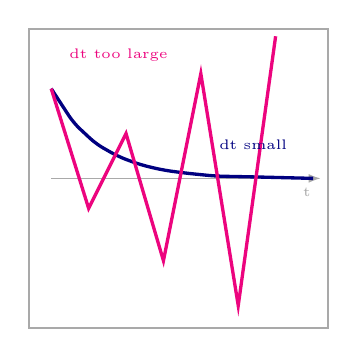
\begin{tikzpicture}[scale=0.95]
  \draw[DarkGray,thick] (0,0) rectangle (4,4);
  \draw[DarkGray,-{Latex[length=1.5mm]}] (0.3,2) -- (3.9,2) node[below left,font=\tiny] {t};
  \draw[NavyBlue,very thick,rounded corners=3pt] (0.3,3.2) -- (0.6,2.74) -- (0.9,2.46) -- (1.2,2.29) -- (1.5,2.18) -- (1.8,2.11) -- (2.1,2.07) -- (2.5,2.03) -- (3.0,2.02) -- (3.8,2.0);
  \draw[RubineRed,very thick] (0.3,3.2) -- (0.8,1.6) -- (1.3,2.6) -- (1.8,0.9) -- (2.3,3.4) -- (2.8,0.3) -- (3.3,3.9);
  \node[font=\tiny,NavyBlue] at (3.0,2.45) {dt small};
  \node[font=\tiny,RubineRed] at (1.2,3.65) {dt too large};
\end{tikzpicture}}
\end{frame}

% ---------------------------------------------------------------- goals, sources
\begin{frame}{What you will be able to do after this chapter}
\label{fr:goals}
\footnotesize
\begin{itemize}
  \item Say what convergence, order and stability mean for a numerical method, and tell an unstable run from an inaccurate one.
  \item Reproduce the course's two warm-ups: Euler's method on $y' = -15y$ (one multiplier per step decides everything) and the explicit heat equation (stable only for $r = \Delta t/\Delta x^2 \le 1/2$; convergence in space and in time; the order measured).
  \item Blow up IB2d's rubber band two ways on purpose (a time step of 1, a band 1000 times stiffer), read the error each port gives, and map which stiffness--time-step pairs survive.
  \item Refine an IB2d example properly: the points stay at $\Delta s \approx \Delta x/2$, \code{input2d} and the generator agree, the spring constant is rescaled so the band is the same band; then measure how fast the answer converges and what it costs.
  \item Run the lab in Python on a laptop (\code{examples/IB2d/Stability\_Lab}: a generator with the grid and stiffness as arguments, a sweep script, an analysis script) and write the same protocol for an example of your own.
\end{itemize}
\begin{punchbox}
\small Everything measured here ran in October 2026 with the Python IB2d on a laptop (73 runs, most 2--90 s; the $256^2$ runs 3--8 minutes). The numbers are in the tables; the scripts that made them are in the repository, so the tables can be remade on another machine.
\end{punchbox}
\end{frame}

\begin{frame}{Where this chapter comes from}
\label{fr:sources}
\footnotesize
\begin{itemize}
  \item \al{``Lecture 19: Stability and convergence'' (UA course, 2021, edited 2023; 40 slides):} the three ideas, Euler's method by hand and in \code{stiff\_ode\_example.m}, the CFL condition, the heat equation in \code{heat\_equation.m} (space, then time), rate and order of convergence, the IB rules of thumb, and the homework-5 lab on the rubber band (blow it up with $\Delta t$, blow it up with stiffness, refine $32 \to 64$). The only stability lab in twelve years of material.
  \item \al{Lecture 12 (2021--23), its numerics block (slides 8--21):} the same ideas in short form, plus ``IBAMR instabilities'': the time step needed is inversely proportional to the force applied, the forcing term (not CFL) is what blows up, so avoid large accelerations and very stiff springs.
  \item \al{The MATLAB exercise files} (\code{stiff\_ode\_example.m}, \code{heat\_equation.m}): in the repository under \code{examples/support/matlab-exercises}, corrected, with Python versions that give the same numbers (chapter 5 runs them; the Octave-against-Python check is in the folder's README, Appendix A).
  \item \al{The course's remote-desktop route} (UA's VCAT virtual lab, MATLAB, downloading IB2d): kept on one slide; chapters 1 and 4a are the current set-up.
\end{itemize}
What is new here: every figure remade from the scripts; the measured orders; the IB2d lab rewritten for the Python port with a parametrised generator, a 41-run stiffness--time-step map, a five-grid refinement with the tension kept and a four-step time-step study; the area loss of a closed band measured against grid and points per cell (it is the method's, not the spacing's); the inverse relationship checked rather than stated.
\end{frame}

\begin{frame}[fragile]{The course's lab set-up, then and now}
\label{fr:setup}
\begin{columns}[T]
\column{0.5\textwidth}

\includegraphics[width=\textwidth]{ch4d-l19-vcat.png}
\sourcecredit{Lecture 19, slides 7--10 (2021): UA's VCAT virtual computer lab (apporto) with MATLAB; IB2d downloaded from GitHub as a zip.}
\column{0.48\textwidth}
\footnotesize
\al{Then (2021):} log in to VCAT with a NetID (``this might take a while the first time''), launch MATLAB, download and extract \code{ib2d.zip} to Documents or the Desktop, download VisIt from \url{https://visit-dav.github.io/visit-website/releases-as-tables/#latest}, make a \code{MATH481/HW5} folder with \code{heat\_equation.m} and \code{stiff\_ode\_example.m}, unzip \code{Rubberband\_HW5} into \code{Example\_Standard\_Rubberband}, and change MATLAB's folder to it (or type the path).

\al{Now:} the two exercise files and the rubber band are in this repository (\code{examples/support/matlab-exercises}, \code{examples/IB2d/Stability\_Lab}); IB2d in MATLAB or Python as in chapter 4a; VisIt as in chapter 4b; Puma as in chapter 1. The VCAT route still exists (\url{https://it.arizona.edu/documentation/vcat-how-tos}) for a machine without MATLAB.
\end{columns}
\end{frame}

% ---------------------------------------------------------------- the three ideas
\begin{frame}{Numerical analysis: three ideas}
\label{fr:ideas}
\small
Numerical analysis is not only the design of numerical methods but also their analysis. Three central concepts:
\begin{itemize}
  \item \al{convergence}: whether the method approximates the solution (the numerical solution approaches the exact one as the step size $h \to 0$),
  \item \al{order}: how well it approximates the solution (how fast the error shrinks with $h$),
  \item \al{stability}: whether errors are damped out.
\end{itemize}
\begin{punchbox}
\small \al{Numerical instability.} Typically an algorithm would approach the right solution in the limit if there were no round-off or truncation errors; but depending on the method, errors can be magnified instead of damped, and the error grows exponentially. An unstable run is not ``a bit off'': it is garbage after a few steps, and usually ends with \code{NaN} or an error.
\end{punchbox}
\small
Two things to keep apart from the start: a \al{stable but inaccurate} run (coarse grid, large but admissible step: smooth, wrong numbers) and an \al{unstable} run (oscillations that grow, then overflow). The first is fixed by refinement; the second by a smaller step or a softer force, as the lab shows.
\end{frame}

\begin{frame}{The motivating example: $y' = -15y$}
\label{fr:motivate}
\small
Consider the initial value problem
\[ y'(t) = -15\,y(t), \qquad t \ge 0,\ y(0) = 1, \qquad\text{with exact solution}\qquad y(t) = e^{-15t} \to 0 \text{ as } t \to \infty. \]
We seek a numerical solution that exhibits the same behaviour. The figure in the lecture (reproduced on slide \ref{fr:eulerfig}) illustrates the numerical issues for integrators applied to this equation:
\begin{enumerate}
  \item Euler's method with step size $h = 1/4$ oscillates wildly and quickly exits the range of the graph;
  \item Euler's method with half the step size, $h = 1/8$, produces a solution within the graph boundaries, but oscillates about zero;
  \item the trapezoidal method (the two-stage Adams--Moulton method)
  \[ y_{n+1} = y_n + \tfrac12 h\,\big(f(t_n, y_n) + f(t_{n+1}, y_{n+1})\big) \]
  gives a much better result (slide \ref{fr:trap}).
\end{enumerate}
The equation is \al{stiff}: its own time scale ($1/15$) is far shorter than the interval you care about ($t$ up to 1), so the step size is dictated by stability, not by the accuracy you would need to draw $e^{-15t}$.
\sourcecredit{Lecture 19, slide 5 (the text of its figure).}
\end{frame}

\begin{frame}{Euler's method by hand: $h = 1/4$}
\label{fr:byhand}
\begin{columns}[T]
\column{0.52\textwidth}
\footnotesize
$y'(t) = -15\,y(t) = f(t, y(t))$, $y(0) = 1$. Let $h = \tfrac14$.
\begin{align*}
 y_1 &= y_0 + h\,f(t_0, y_0) = y_0 + h\,(-15 y_0) \\
     &= 1 + \tfrac14 (-15 \cdot 1) \\
     &= 1 - \tfrac{15}{4} = -2.75 \\[2pt]
 y_2 &= y_1 + h\,f(t_1, y_1) = y_1 + h\,(-15 y_1) \\
     &= -2.75 + \tfrac14 (-15 \cdot (-2.75)) \\
     &= 7.5625 \\[2pt]
 y_3 &= -20.796875, \qquad y_4 = 57.19140625
\end{align*}
The exact solution at those times: $0.0235$, $0.00055$, $1.3 \cdot 10^{-5}$, $3.1 \cdot 10^{-7}$.
\column{0.46\textwidth}
\footnotesize
\al{Why.} Each step multiplies $y$ by the same number:
\[ y_{n+1} = y_n - 15 h\, y_n = (1 - 15h)\, y_n, \]
\[ y_n = (1-15h)^n. \]
\begin{itemize}
  \item $|1 - 15h| < 1 \iff 0 < h < \tfrac{2}{15} = 0.133$: the method decays (stable);
  \item $-1 < 1 - 15h < 0 \iff \tfrac{1}{15} < h < \tfrac{2}{15}$: decays, but changes sign every step;
  \item $h > \tfrac{2}{15}$: $|1-15h| > 1$, growth by that factor per step. At $h = 1/4$ the factor is $-2.75$.
\end{itemize}
For $y' = \lambda y$ in general the factor is $1 + h\lambda$; Euler is stable where $|1 + h\lambda| < 1$, the disc of radius 1 about $-1$ in the complex $h\lambda$ plane. A stiff system is one whose fastest $\lambda$ sets $h$.
\end{columns}
\end{frame}

\begin{frame}[fragile]{\code{stiff\_ode\_example.m}, as handed out}
\label{fr:stiffcode}
\begin{columns}[T]
\column{0.5\textwidth}
\begin{lstlisting}[style=mtiny]
function stiff_ode_example(dt, tfinal)
% This example numerically solves the stiff ode y'(t) = -15*y(t) using Euler's
% method. This has an exact solution given by y(t) = exp(-15*t). The inputs
% are dt, the time step size, and tfinal, the final simulation time.

N = ceil(tfinal/dt);    %Determine the number of time steps
y = zeros(N);           %Initialize y to hold the numerical solution
y_exact = zeros(N);     %Initialize y_exact to hold the exact solution
time = zeros(N);        %Initialize time to hold the times

y(1) = 1;               %Initial conditions
y_exact(1) = 1;
time(1) = 0;
\end{lstlisting}
\column{0.48\textwidth}
\begin{lstlisting}[style=mtiny]
%Loop through all time steps and calculate y using Euler's method
for i = 2:N,
  y(i)= y(i-1)+dt*(-15*y(i-1));
  time(i)=(i-1)*dt;                 %update time
  y_exact(i) = exp(-15*time(i));    %save exact solution
end

%graph the numerical and the exact solutions
hold off
plot(time, y, '-b');
hold on
plot(time, y_exact, '-r');
xlabel('time');
ylabel('y');
legend('Eulers method', 'Exact solution');
\end{lstlisting}
\footnotesize
Call it as \code{stiff\_ode\_example(dt, tfinal)} and try \code{(0.2, 1)}, \code{(0.1, 1)}, \code{(0.01, 1)} to observe the instability.
\end{columns}
\sourcecredit{Lecture 19, slides 13--16. The repository's copy has two corrections (slide \ref{fr:stiffbugs}); \code{stiff\_ode\_example.py DT TFINAL} is the Python version.}
\end{frame}

\begin{frame}{Six time steps for $y' = -15y$}
\label{fr:eulerfig}
\centering
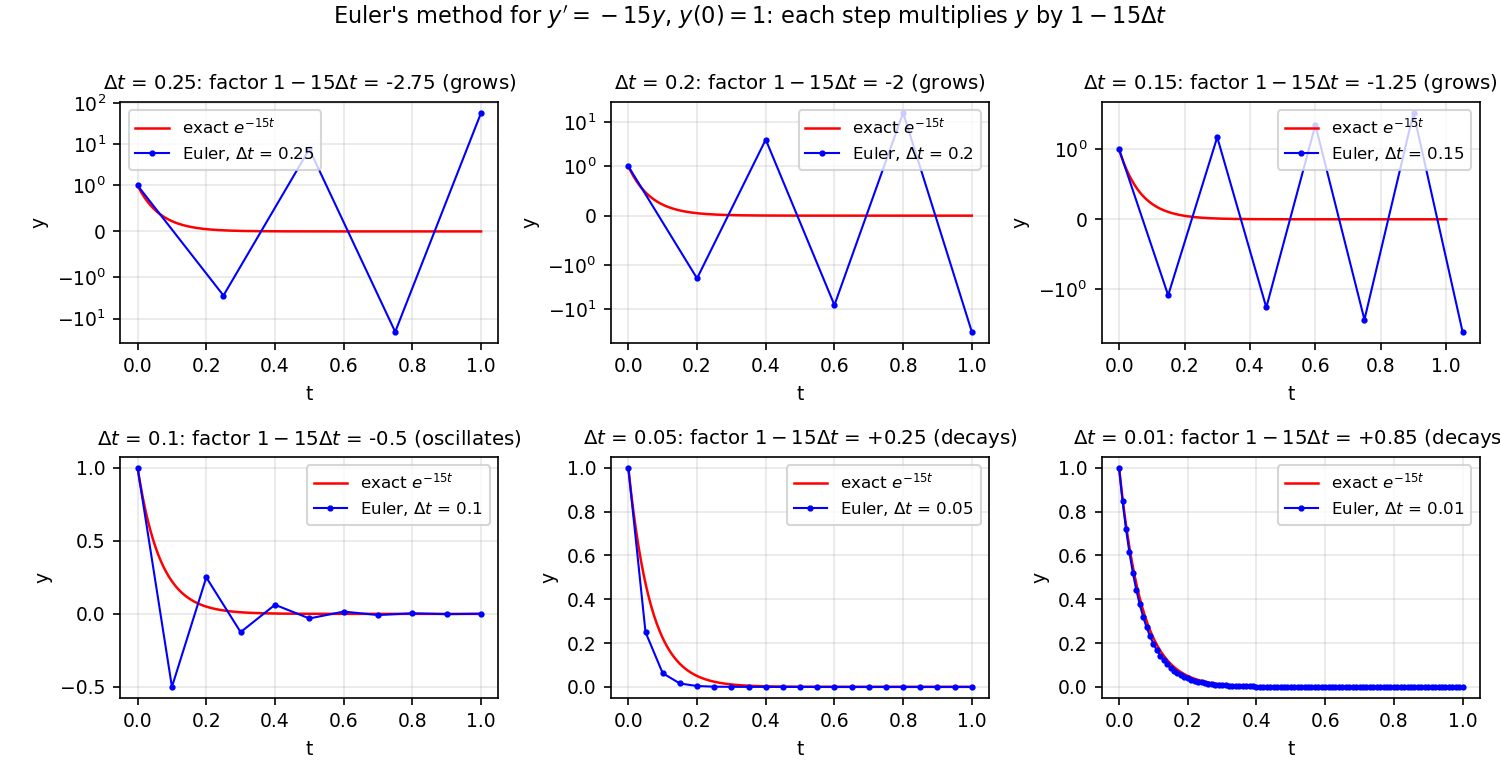
\includegraphics[width=0.64\textwidth]{ch4d-euler.png}

\tiny
\resizebox{0.96\textwidth}{!}{%
\begin{tabular}{@{}lllll@{}}
\toprule
$\Delta t$ & factor $1 - 15\Delta t$ & behaviour & the lab's three & \\
\midrule
0.25 & $-2.75$ & grows, alternating ($y_4 = 57$) & & the hand calculation \\
0.2 & $-2$ & grows, alternating ($y = 16$ at $t = 0.8$, $-32$ at $t = 1$) & \code{(0.2, 1)} & ``exits the range of the graph'' (said of $h = 1/4$ on slide \ref{fr:motivate}) \\
0.15 & $-1.25$ & grows slowly ($\pm 4$ at $t = 1$) & & just outside $2/15$ \\
0.1 & $-0.5$ & decays, changes sign every step & \code{(0.1, 1)} & ``oscillates about zero'' (said of $h = 1/8$) \\
0.05 & $+0.25$ & decays, too fast at first & & \\
0.01 & $+0.85$ & follows $e^{-15t}$ & \code{(0.01, 1)} & \\
\bottomrule
\end{tabular}}
\sourcecredit{\code{tools/ch4d\_figures.py} with \code{stiff\_ode\_example.py}; the top row uses a symmetric log axis so that the growth fits.}
\end{frame}

\begin{frame}{The course's own picture, and the sketch it started from}
\label{fr:eulerold}
\begin{columns}[T]
\column{0.5\textwidth}
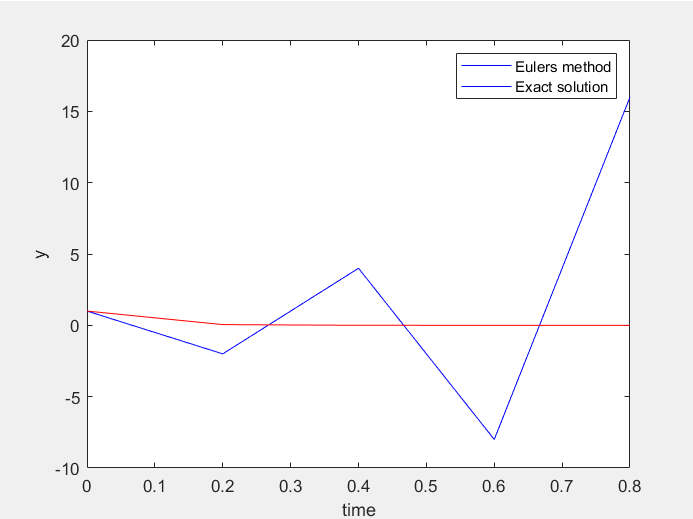
\includegraphics[width=0.92\textwidth]{ch4d-l19-euler-matlab.png}
\sourcecredit{Lecture 19, slide 17: MATLAB, \code{stiff\_ode\_example(0.2, 1)}. The blue curve reaches $16$ at $t = 0.8$; the plot stops there because of the second bug of slide \ref{fr:stiffbugs}.}
\column{0.48\textwidth}
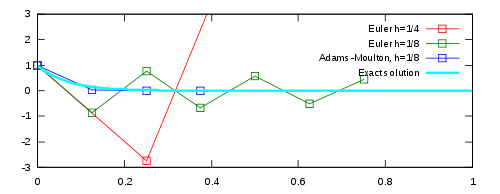
\includegraphics[width=0.92\textwidth]{ch4d-l19-sketch.png}
\sourcecredit{Lecture 19, slides 13 and 16: the sketch of the three behaviours (red grows, green oscillates, blue follows the cyan exact curve).}
\end{columns}
\small
Read the MATLAB plot against the table: $\Delta t = 0.2$ gives the factor $-2$, so $y = 1, -2, 4, -8, 16$ at $t = 0, 0.2, \ldots, 0.8$. That is the whole phenomenon: not ``errors accumulate'', but ``errors are multiplied by 2 every step''.
\end{frame}

\begin{frame}{Two bugs in the handed-out \code{stiff\_ode\_example.m}}
\label{fr:stiffbugs}
\small
\begin{itemize}
  \item \al{\code{zeros(N)} makes an $N \times N$ matrix}, not a vector of length $N$. \code{y}, \code{y\_exact} and \code{time} were all $N \times N$; the loop filled their first columns and \code{plot(time, y)} drew $N$ curves, $N - 1$ of them the all-zero columns, i.e. $N$ points on top of each other at the origin, invisible. The visible damage is to the legend, whose two labels go to the first two of the $2N$ line objects: in the course's plot (slide \ref{fr:eulerold}) ``Exact solution'' is drawn in the blue of the Euler curve and the red exact curve has no entry. The repository's copy uses \code{zeros(1, N)}.
  \item \al{The time grid stops one step short of \code{tfinal}}: with \code{N = ceil(tfinal/dt)} and the loop \code{for i = 2:N}, the last time is \code{(N-1)*dt}; for \code{(0.2, 1)} that is $0.8$, as the picture shows. The copy uses \code{N = ceil(tfinal/dt) + 1} time levels so that the last is at (or just past) \code{tfinal}.
\end{itemize}
Neither changes the numbers that matter (the first column of \code{y} was right), which is how both survived unnoticed for years. The Python version (\code{stiff\_ode\_example.py}) is a vector version of the corrected file; Octave and Python agree to the last digit for $\Delta t = 0.05$ and $0.15$ (the check is recorded in the README of \code{examples/support/matlab-exercises}, Appendix A; chapter 5 runs the same three cases).
\begin{punchbox}
\small A good habit from this: check \code{size(y)} after the initialisation, and print the last time value before you trust a plot's right edge.
\end{punchbox}
\end{frame}

\begin{frame}{The trapezoidal method does not have this problem}
\label{fr:trap}
\small
The two-stage Adams--Moulton (trapezoidal) method of slide \ref{fr:motivate}, applied to $y' = \lambda y$:
\[ y_{n+1} = y_n + \tfrac{h}{2}\big(\lambda y_n + \lambda y_{n+1}\big) \quad\Longrightarrow\quad y_{n+1} = \frac{1 + h\lambda/2}{1 - h\lambda/2}\; y_n . \]
For $\lambda = -15$ the factor is $(1 - 7.5h)/(1 + 7.5h)$, which has modulus below 1 for \emph{every} $h > 0$: the method is \al{A-stable}. With $h = 1/4$ the factor is $-0.304$ (it still changes sign, but decays); with $h = 1/8$ it is $+0.032$ (positive: no sign change any more, which is why the blue curve of the lecture's sketch, slide \ref{fr:eulerold}, hugs the exact one).
\begin{itemize}
  \item The price: the new value appears on both sides (an \al{implicit} method). Here it is one division; for a nonlinear $f$ it is a solve at every step.
  \item IB2d and IBAMR treat the fluid's viscous term implicitly (that is why the viscous time-step limit $\Delta t < \Delta x^2/(4\nu)$ does not bite) and the boundary force \al{explicitly}: the force is evaluated at the known positions and then the points are moved. The force is the stiff part, so it sets $\Delta t$ (slide \ref{fr:cfl}); an implicit IB method is a research topic, not a switch.
  \item Exercise \ref{fr:exercises}: add the trapezoidal step to \code{stiff\_ode\_example} and repeat the three runs.
\end{itemize}
\end{frame}

\begin{frame}{The CFL condition, and why it is not what limits an IB run}
\label{fr:cfl}
\small
The Courant--Friedrichs--Lewy condition is a necessary condition for stability when certain PDEs (usually hyperbolic ones) are solved by finite differences. The general CFL condition for the $n$-dimensional case:
\[ C = \Delta t \sum_{i=1}^{n} \frac{u_{x_i}}{\Delta x_i} \le C_{\max}, \qquad \text{typically } C_{\max} = 1 : \]
in one step, information may not travel further than one cell. In immersed boundary simulations we rarely have to worry about this. The lecture's reason (Lecture 12, ``IBAMR instabilities''):
\begin{itemize}
  \item instabilities typically occur when the time step is too big;
  \item the time step necessary for stability is \al{inversely proportional to the force applied to the fluid};
  \item the forcing term is typically what causes the instability (not the CFL condition);
  \item strategy: avoid large forces by minimising accelerations and very stiff springs.
\end{itemize}
The lab checks the second point on the rubber band (slide \ref{fr:map}): $\Delta t_{\max}$ does fall as the stiffness rises. The CFL number of a typical IB run is small anyway: at $512^2$ with $\Delta t = 10^{-5}$ and $u \sim 1$, $C = 0.005$.
\sourcecredit{Lecture 19, slide 18; Lecture 12, slides 12--13.}
\end{frame}

\begin{frame}{Convergence}
\label{fr:convergence}
\small
A numerical method is \al{convergent} if the numerical solution approaches the exact solution as the step size $h \to 0$. In the immersed boundary method you typically need to worry about convergence \al{in space}: is the flow around the boundary well resolved? Are shed vortices well resolved?
\begin{itemize}
  \item Convergence is checked by running the same problem at two or three resolutions and watching a number you care about settle (a force, a flow rate, a position). The lab does this for the band's shape (slides \ref{fr:gridtab} and \ref{fr:dttab}).
  \item Stability and convergence are linked (for linear problems, consistency + stability = convergence, the Lax equivalence theorem), which is why an unstable scheme cannot be ``fixed'' by refining: the heat equation at $r > 1/2$ gets worse with every extra step, not better.
  \item The order (slide \ref{fr:order}) tells how much a refinement buys: halving $h$ divides the error by $2^p$. The IB method is second order away from the boundary and first order at it (slide \ref{fr:rules}), so an IB answer typically converges with $p$ between 1 and 2.
\end{itemize}
\sourcecredit{Lecture 19, slide 19; Lecture 12, slide 14.}
\end{frame}

% ---------------------------------------------------------------- the heat equation
\begin{frame}{The heat equation: a model with both issues at once}
\label{fr:heat}
\begin{columns}[T]
\column{0.5\textwidth}
\footnotesize
To look at an example that incorporates issues of instability and convergence in space and time, we simulate the heat equation. Let $u(x,t)$ give the temperature at time $t$ and position $x$ along a bar:
\[ u_t = D\,u_{xx},\quad 0 < x < 1, \]
\[ u(0,t) = u(1,t) = 0,\quad u(x,0) = \sin 2\pi x, \]
with $D = 1$. Intuitively this is the heat distribution on a bar with hot spots; over time the heat diffuses. Exact solution: $u = e^{-4\pi^2 t} \sin 2\pi x$.

\al{The scheme} (explicit, forward in time, central in space): with $x_j = j\,\Delta x$, $\Delta x = 1/(n+1)$, $\Delta t = 0.1/T$,
\[ u_j^{m+1} = r\,u_{j-1}^m + (1 - 2r)\,u_j^m + r\,u_{j+1}^m,\quad r = \frac{\Delta t}{\Delta x^2}. \]
\column{0.48\textwidth}
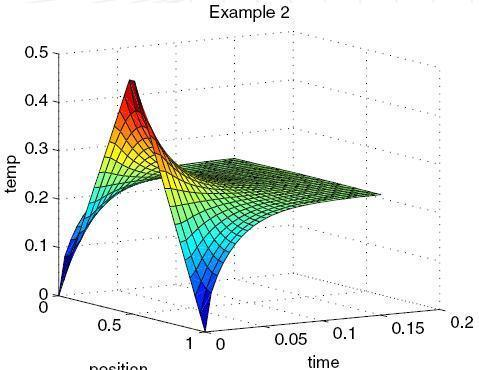
\includegraphics[width=0.9\textwidth]{ch4d-l19-heat-surface.jpg}
\sourcecredit{Lecture 19, slide 21: $u(x,t)$ for a different initial condition (a single tent-shaped hot spot, followed to $t = 0.2$).}
\small The script plots the analytical and numerical solutions at a single time, $t = 0.1$, for $n$ interior points and $T$ time steps: \code{heat\_equation(n, T)}.
\end{columns}
\end{frame}

\begin{frame}[fragile]{\code{heat\_equation.m}, as handed out}
\label{fr:heatcode}
\begin{columns}[T]
\column{0.5\textwidth}
\begin{lstlisting}[style=mtiny]
function heat_equation(n,T)
% function Example4_1(n,T)
% solve Ut=Uxx, U(0,t)=U(1,t)=0, U(0,x)=sin(3*pi*x).
%    n: n+1 is the number of intervals in x-direction,
%    T: the no. of intervals in t-dir.
clf,
t=0.1; dt=t/T; dx=1/(n+1);
r=dt/(dx*dx);
x=[dx:dx:1-dx]; % all the inner points
%analytical solution when t=0.1:
ex=[0:0.005:1];
u_ex=exp(-4*(pi*pi)*t)*sin(2*pi*ex);
%up is the previous solution and un is the next solution.
up=zeros(size(x)); un=zeros(size(x));
%initial condition:
up=sin(2*pi*x);
\end{lstlisting}
\column{0.48\textwidth}
\begin{lstlisting}[style=mtiny]
%the calculating loop:
for m=1:T,
  for j=2:n-1,
    un(j) = r*up(j-1)+(1-2*r)*up(j)+r*up(j+1);
  end,
%take care of boundary conditions:
  un(1)=(1-2*r)*up(1)+r*up(2);
  un(n)=r*up(n-1)+(1-2*r)*up(n);
%put un into up:
  up=un;
end,
p=plot(ex,u_ex,[0 x 1],[0 up 0],'--',[0 x 1],[0 up 0],'o');
h=text(0.01,-0.017,sprintf('dx=%6.3g, dt=%g, r=%g',dx,dt,r));
set(p,'LineWidth',1.2), set(h,'FontSize',18),
print -deps Example4_1.eps
\end{lstlisting}
\end{columns}
\footnotesize
One thing fixed in the repository's copy: the header said $\sin 3\pi x$ (and \code{U(0,x)}) where the code and the exact solution use $\sin 2\pi x$ at $t = 0$. Two things left as they were, so you will meet them: the name in the comment, \code{Example4\_1}, is from an older course, and \code{print -deps} writes \code{Example4\_1.eps} into the current folder on every call (delete the line if you do not want the file). The Python version is \code{heat\_equation.py N T} (vectorised loop, PNG output, same numbers to $10^{-9}$ or better: the README of \code{examples/support/matlab-exercises}, Appendix A; chapter 5 runs them).
\sourcecredit{Lecture 19, slides 22--24.}
\end{frame}

\begin{frame}{Convergence in space: $T = 100$, $n = 3, 5, 10, 20$}
\label{fr:heatspace}
\begin{columns}[T]
\column{0.56\textwidth}
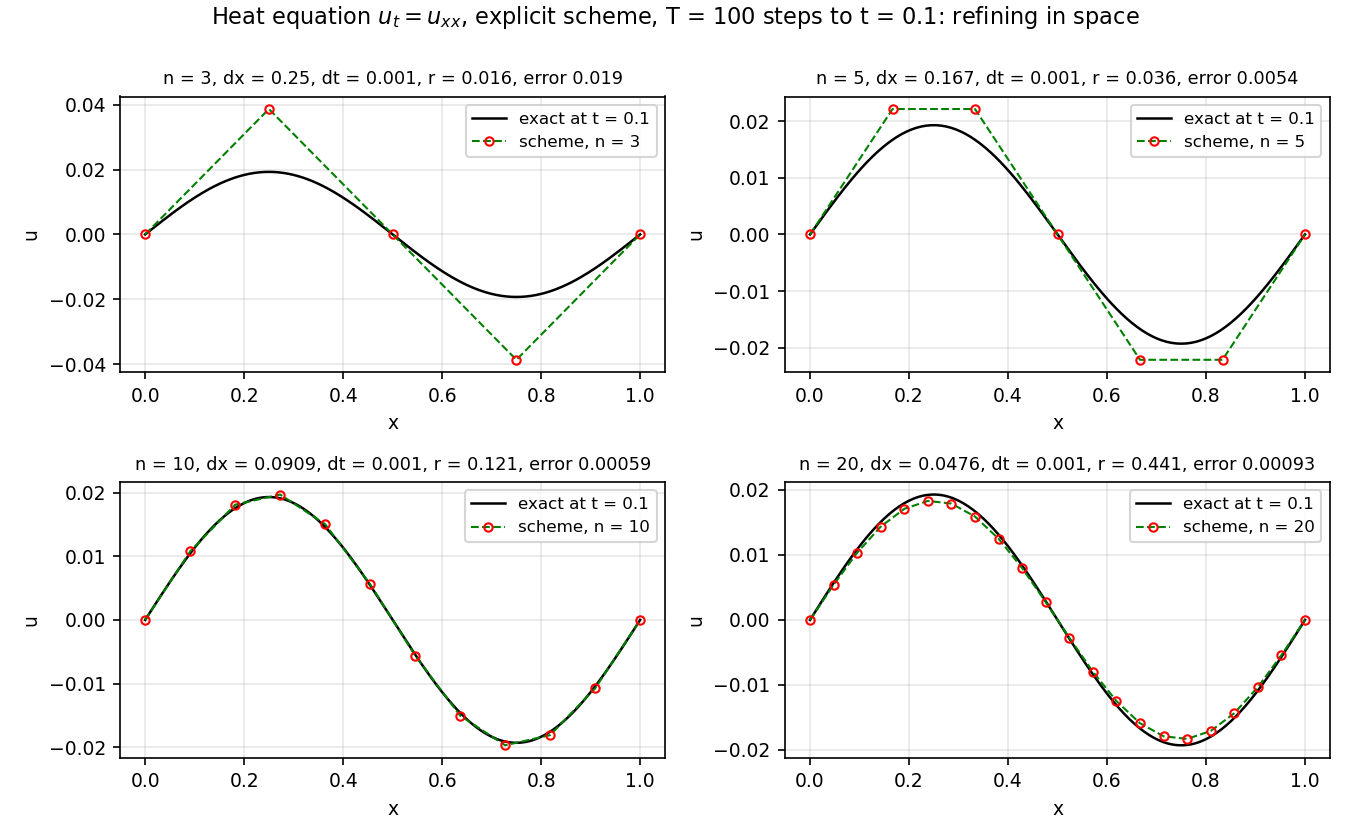
\includegraphics[width=\textwidth]{ch4d-heat-space.png}
\column{0.42\textwidth}
\scriptsize
\begin{tabular}{@{}rllll@{}}
\toprule
$n$ & $\Delta x$ & $r$ & max error \\
\midrule
3 & 0.25 & 0.016 & $1.9 \cdot 10^{-2}$ \\
5 & 0.167 & 0.036 & $5.4 \cdot 10^{-3}$ \\
10 & 0.091 & 0.121 & $5.9 \cdot 10^{-4}$ \\
20 & 0.048 & 0.441 & $9.3 \cdot 10^{-4}$ \\
\bottomrule
\end{tabular}

\footnotesize
The lab: set $T = 100$ and try $n = 3, 5, 10, 20$ to show convergence in space. The curves do converge to the exact one; the error falls by 3.6 from $n = 3$ to 5 and by 9 from 5 to 10, more than the 2.3 and 3.4 a second-order scheme would give for those $\Delta x$ ratios (slide \ref{fr:orderfig} measures the clean $p = 2$ with $r$ held fixed; here $r$ is climbing towards the cancelling value $1/6$ of slide \ref{fr:sixth}).
\end{columns}
\sourcecredit{\code{tools/ch4d\_figures.py} with \code{heat\_equation.py}; the errors are the maximum over the interior points at $t = 0.1$.}
\end{frame}

\begin{frame}{The surprise: $n = 20$ is worse than $n = 10$}
\label{fr:heatsurprise}
\small
\al{The surprise:} $n = 20$ is \emph{worse} than $n = 10$. With $\Delta t$ fixed at $10^{-3}$ the time error does not shrink ($\Delta t/2 = 5 \cdot 10^{-4}$), while the space error falls below it between $n = 10$ ($\Delta x^2/12 = 6.9 \cdot 10^{-4}$) and $n = 20$ ($1.9 \cdot 10^{-4}$); the two have opposite signs (slide \ref{fr:order}: the leading error is $(\Delta t/2 - \Delta x^2/12)\,u_{xxxx}$), so they partly cancel at $n = 10$ and the time error is left standing at $n = 20$. Refining one of $\Delta x$, $\Delta t$ alone does not always help; refine both.

\begin{punchbox}
\small The table of slide \ref{fr:heatspace}: $5.9 \cdot 10^{-4}$ at $n = 10$, $9.3 \cdot 10^{-4}$ at $n = 20$, both with $\Delta t = 10^{-3}$. Slide \ref{fr:sixth} shows the same effect from the other side, with $n$ fixed and $\Delta t$ varied.
\end{punchbox}
\end{frame}

\begin{frame}{The time step: $n = 10$, $T = 2, 4, 8, 16, 32, 64$}
\label{fr:heattime}
\begin{columns}[T]
\column{0.58\textwidth}
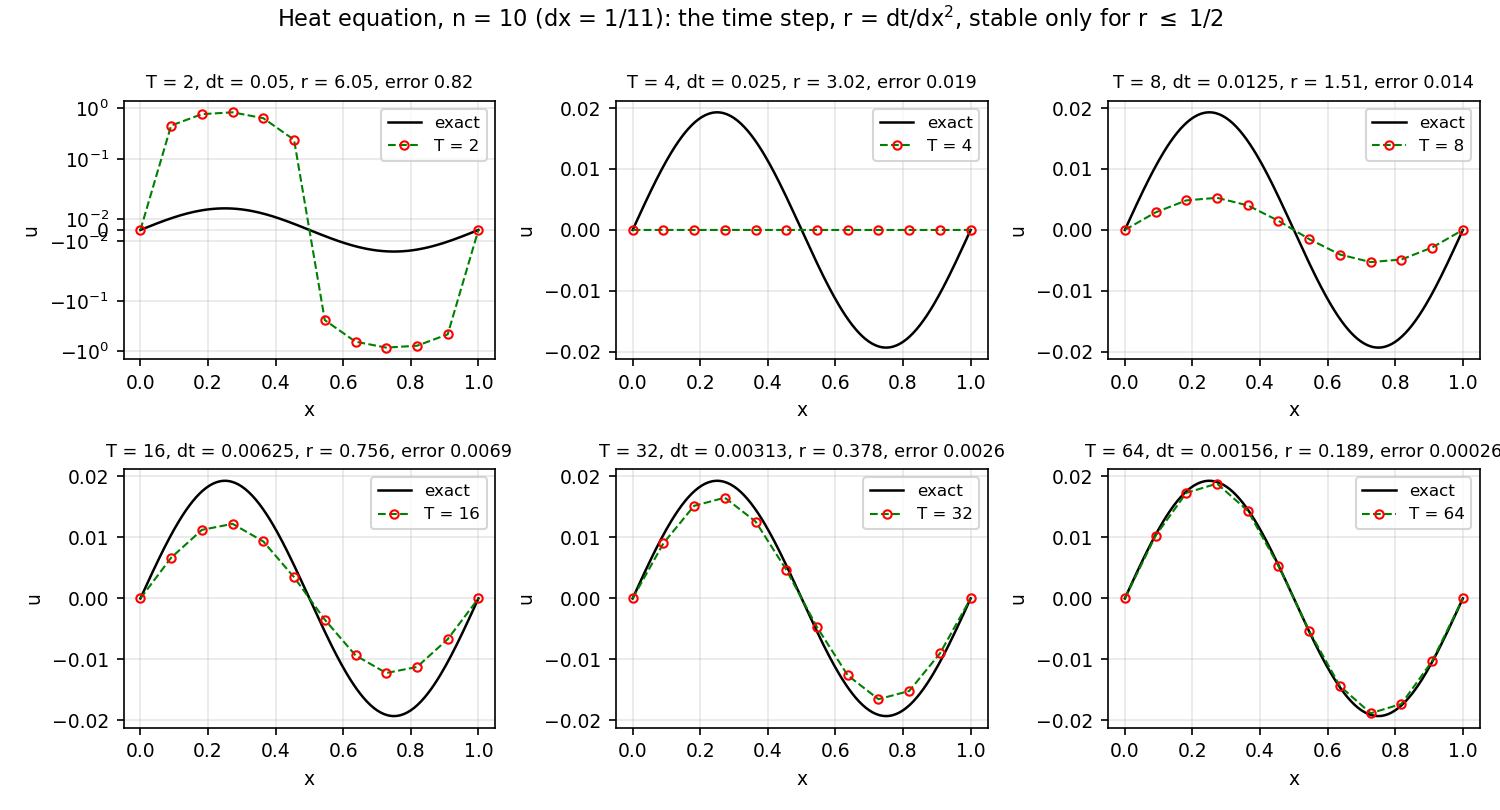
\includegraphics[width=\textwidth]{ch4d-heat-time.png}
\column{0.40\textwidth}
\tiny
\begin{tabular}{@{}rlllp{1.5cm}@{}}
\toprule
$T$ & $\Delta t$ & $r$ & error & \\
\midrule
2 & 0.05 & 6.05 & 0.82 & a sine 44 times too large \\
4 & 0.025 & 3.02 & 0.019 & wiped to $2 \cdot 10^{-6}$ \\
8 & 0.0125 & 1.51 & 0.014 & too small \\
16 & 0.00625 & 0.756 & 0.0069 & unstable, not yet visible \\
32 & 0.0031 & 0.378 & 0.0026 & stable \\
64 & 0.0016 & 0.189 & 0.00027 & stable \\
\bottomrule
\end{tabular}

\scriptsize
The lab: set $n = 10$ and try $T = 2, 4, 8, 16, 32, 64$; the run goes to $t = 0.1$, so $\Delta t = 0.1/T$ and $r = 12.1/T$. Four of the six are above the limit $r = 1/2$. $T = 2$ keeps 85\,\% of the initial sine after two steps where 2\,\% should be left (its multiplier is $-0.92$ per step: slide \ref{fr:vonneumann}), a smooth curve 44 times too large; $T = 4$ wipes the solution out (the sine's multiplier $1 - 4r\sin^2(\pi/11) = 0.04$ at $r = 3.02$: one step removes 96\,\% of it); $T = 8$ decays too fast (0.52 per step); $T = 16$ at $r = 0.756$ \emph{looks} fine, and is not: slide \ref{fr:vonneumann}.
\end{columns}
\sourcecredit{\code{tools/ch4d\_figures.py}; the first panel has a symmetric log axis.}
\end{frame}

\begin{frame}{Why $r \le 1/2$, and the unstable run that looks fine}
\label{fr:vonneumann}
\footnotesize
Put a single Fourier mode $u_j^m = g^m e^{i\theta j}$ into the scheme ($\theta = k\,\Delta x$):
\[ g = 1 - 2r + 2r\cos\theta = 1 - 4r\sin^2\tfrac{\theta}{2}, \qquad |g| \le 1 \text{ for all } \theta \iff r \le \tfrac12 . \]
The most dangerous mode is the sawtooth $\theta = \pi$ (alternating signs from point to point), with $g = 1 - 4r$: it is multiplied by $|1 - 4r|$ every step.
\begin{itemize}
  \item $r = 6.05$ ($T = 2$): $g = -23$ for the sawtooth, and the initial sine, $\theta = 2\pi/11$, has $g = -0.92$: after two steps $0.85$ of the sine is still there (the exact solution keeps $0.02$), while the sawtooth, starting from round-off, has grown only $23^2 \approx 540$ times, to $10^{-13}$. The first panel of slide \ref{fr:heattime} is therefore a clean sine 44 times too large, not noise; it would take a dozen steps at this $r$ for the noise to reach order one ($23^{12} \cdot 10^{-16} \approx 2$).
  \item $r = 0.756$ ($T = 16$): $g = -2.02$ for the sawtooth. But the initial condition is a smooth sine, so the sawtooth starts at round-off, $10^{-16}$; after 16 steps it has reached $2^{16} \cdot 10^{-16} \approx 10^{-11}$: invisible. Run the same $r$ for 200 steps and it is $10^{45}$. \al{Unstable does not mean visibly wrong right away.} The same happens in IB runs that ``blow up at $t = 0.8$'' after looking reasonable: the growth started at step 1.
  \item $r = 3.02$ ($T = 4$): $g = -11$ for the sawtooth and $g = 1 - 4r\sin^2(\pi/11) = 0.04$ for the sine: the sine itself is all but wiped out in one step ($0.04^4 = 2.5 \cdot 10^{-6}$ after four), which is why that panel is flat.
\end{itemize}
The rule for the explicit heat equation, $\Delta t \le \Delta x^2/(2D)$, is the one IB2d and IBAMR avoid by treating viscosity implicitly; the boundary force is the term they treat explicitly, and it has an analogous limit (slide \ref{fr:map}).
\end{frame}

\begin{frame}{The course's MATLAB plots}
\label{fr:heatold}
\begin{columns}[T]
\column{0.62\textwidth}
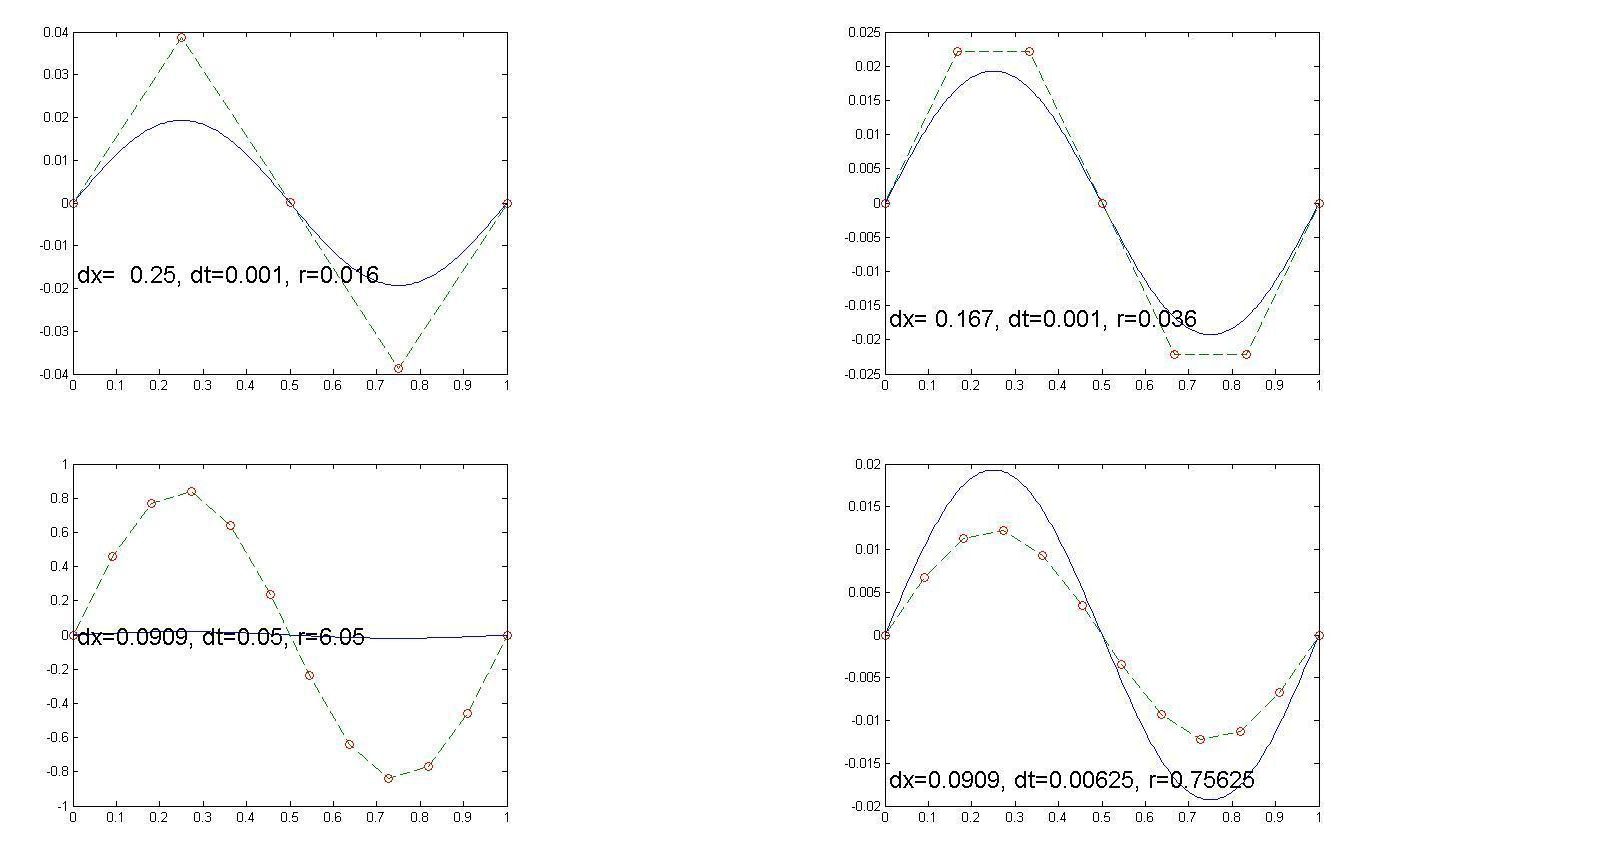
\includegraphics[width=\textwidth]{ch4d-l19-heat-matlab.png}
\sourcecredit{Lecture 19, slides 25--26: $n = 3$ and $5$ at $T = 100$ (top), $T = 2$ and $T = 16$ at $n = 10$ (bottom); the text in each panel is the script's own \code{dx, dt, r} stamp.}
\column{0.36\textwidth}
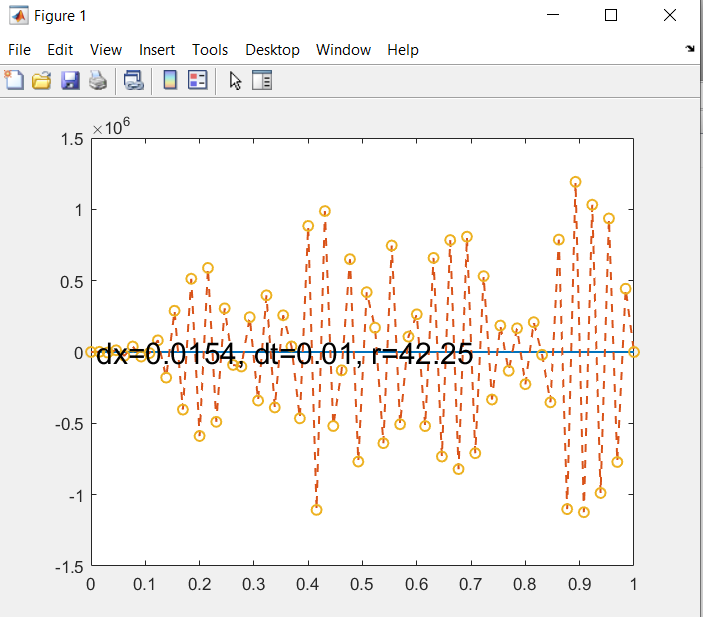
\includegraphics[width=\textwidth]{ch4d-l19-blowup-matlab.png}
\sourcecredit{Lecture 19, slide 27: a blow-up to $\pm 1.2 \cdot 10^6$ (the axis runs to $\pm 1.5 \cdot 10^6$) at $r = 42.25$ ($n = 64$, $T = 10$): the sawtooth mode, alternating from point to point.}
\end{columns}
\small
The bottom-left panel ($T = 2$, $r = 6.05$) is the same as our first panel of slide \ref{fr:heattime} on a linear axis; the bottom-right ($T = 16$) is the ``unstable but not yet visible'' case.
\end{frame}

\begin{frame}{Rate and order of convergence}
\label{fr:order}
\footnotesize
In numerical analysis, the speed at which a convergent sequence approaches its limit is called the \al{rate of convergence}. Suppose that the sequence $\{x_k\}$ converges to the number $L$. It converges \al{linearly} to $L$ if there is a number $\mu \in (0,1)$ with
\[ \lim_{k \to \infty} \frac{|x_{k+1} - L|}{|x_k - L|} = \mu ; \]
$\mu$ is called the rate of convergence. The sequence converges with \al{order $q$} to $L$, for $q > 1$, if
\[ \lim_{k \to \infty} \frac{|x_{k+1} - L|}{|x_k - L|^q} = \mu, \qquad \mu > 0 ; \]
$q = 2$ is quadratic convergence, $q = 3$ cubic (Newton's method is quadratic; that is what these definitions are for).

\al{For a discretisation} the word is used differently: a method has order $p$ when the error is $O(h^p)$. Measure it with three resolutions: $e_h \approx C h^p$ gives
\[ p \approx \log_2 \frac{e_{h}}{e_{h/2}}, \qquad\text{or, without an exact solution,}\qquad p \approx \log_2 \frac{|x_{h} - x_{h/2}|}{|x_{h/2} - x_{h/4}|} . \]
The explicit heat scheme has truncation error $\tau = \big(\tfrac{\Delta t}{2} - \tfrac{\Delta x^2}{12}\big) u_{xxxx} + \ldots$ (using $u_{tt} = u_{xxxx}$): first order in time, second in space, and the two cancel at $r = 1/6$.
\sourcecredit{Lecture 19, slides 28--29.}
\end{frame}

\begin{frame}{Measuring the order on the two warm-ups}
\label{fr:orderfig}
\centering
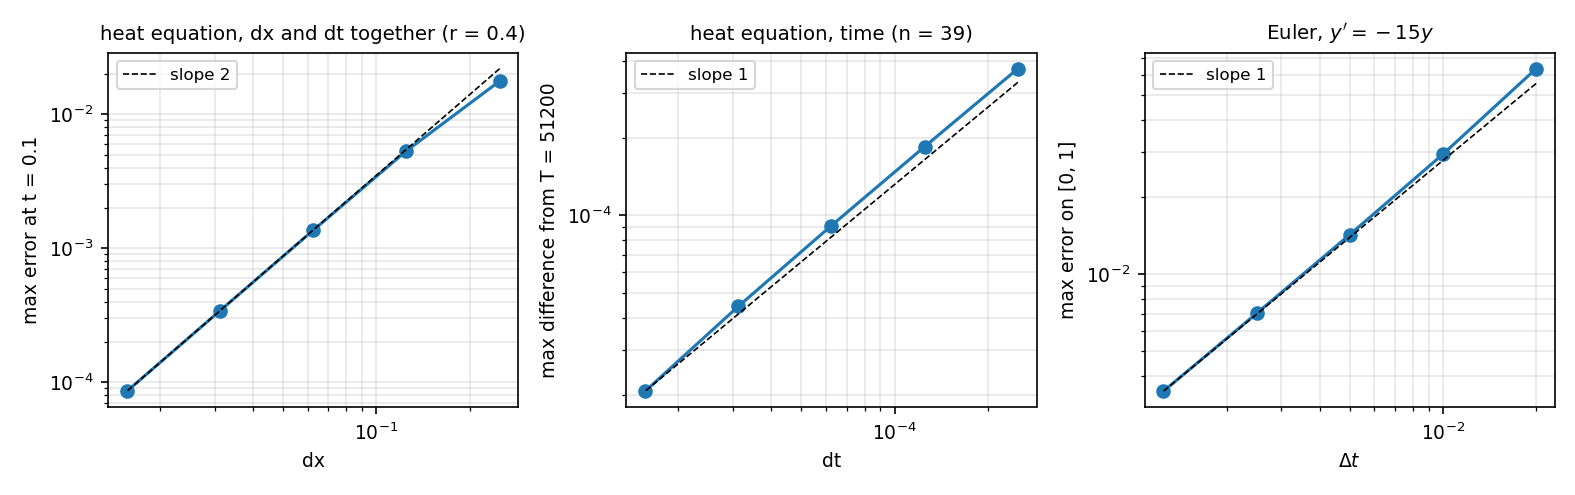
\includegraphics[width=0.9\textwidth]{ch4d-orders.png}

\scriptsize
\begin{tabular}{@{}lllllll@{}}
\toprule
heat, $r = 0.4$ fixed: $\Delta x$ & 1/4 & 1/8 & 1/16 & 1/32 & 1/64 & $p$ = 1.7, 2.0, 2.0, 2.0 \\
max error & $1.8 \cdot 10^{-2}$ & $5.3 \cdot 10^{-3}$ & $1.4 \cdot 10^{-3}$ & $3.4 \cdot 10^{-4}$ & $8.6 \cdot 10^{-5}$ & \\
\midrule
heat, $n = 39$: $\Delta t$ & $2.5 \cdot 10^{-4}$ & $1.25 \cdot 10^{-4}$ & $6.25 \cdot 10^{-5}$ & $3.1 \cdot 10^{-5}$ & $1.6 \cdot 10^{-5}$ & $p$ = 1.0, 1.0, 1.05, 1.1 \\
difference from $T = 51200$ & $3.7 \cdot 10^{-4}$ & $1.9 \cdot 10^{-4}$ & $9.1 \cdot 10^{-5}$ & $4.4 \cdot 10^{-5}$ & $2.1 \cdot 10^{-5}$ & \\
\midrule
Euler, $y' = -15y$: $\Delta t$ & 0.02 & 0.01 & 0.005 & 0.0025 & 0.00125 & $p$ = 1.1, 1.05, 1.0, 1.0 \\
max error on $[0, 1]$ & $6.4 \cdot 10^{-2}$ & $2.9 \cdot 10^{-2}$ & $1.4 \cdot 10^{-2}$ & $7.0 \cdot 10^{-3}$ & $3.5 \cdot 10^{-3}$ & \\
\bottomrule
\end{tabular}
\sourcecredit{Three ways to measure: against the exact solution (left, right), or against a much finer run when there is none (middle), which is how an IB run is measured.}
\end{frame}

\begin{frame}{The $r = 1/6$ cancellation, with numbers}
\label{fr:sixth}
\small
The same script, $n = 79$ ($\Delta x = 1/80$), three time steps:
\begin{center}
\scriptsize
\begin{tabular}{@{}rrrl@{}}
\toprule
$T$ & $\Delta t$ & $r$ & max error at $t = 0.1$ \\
\midrule
2000 & $5 \cdot 10^{-5}$ & 0.32 & $3.6 \cdot 10^{-5}$ \\
4000 & $2.5 \cdot 10^{-5}$ & 0.16 & $1.6 \cdot 10^{-6}$ \\
8000 & $1.25 \cdot 10^{-5}$ & 0.08 & $2.0 \cdot 10^{-5}$ \\
\bottomrule
\end{tabular}
\end{center}
Halving $\Delta t$ from 0.32 to 0.16 improves the answer twenty-fold; halving it again makes it worse. Nothing is wrong: at $r = 1/6$ the first-order time error and the second-order space error cancel, and the scheme is fourth order for that one ratio. The same effect produced the ``$n = 20$ worse than $n = 10$'' row of slide \ref{fr:heatspace} ($r = 0.44$ against $0.12$): with $n = 20$ and $T = 300$ ($r = 0.147$) the error is $6.8 \cdot 10^{-5}$, fourteen times better than at $T = 100$, and at $T = 1000$ ($r = 0.044$) it is $4.2 \cdot 10^{-4}$ again.
\begin{punchbox}
\small Lesson for the IB runs: when a refinement makes a number worse, do not conclude that the code is wrong or that the coarse run was right. Error terms of opposite sign exist; look at three resolutions, not two, and refine space and time together.
\end{punchbox}
\end{frame}


% ---------------------------------------------------------------- IB2d
\begin{frame}{Stability and convergence in IB2d: describing the boundary}
\label{fr:describing}
\begin{columns}[T]
\column{0.55\textwidth}
\footnotesize
In the immersed boundary method, boundaries are always elastic:
\begin{itemize}
  \item they can be stiff enough that they act like rigid objects;
  \item they can be moved in prescribed ways using target points (chapter 4c);
  \item boundaries have been modelled to resist bending, stretching and twisting;
  \item all of these properties can change in time in prescribed ways or according to other models.
\end{itemize}
\al{Immersed boundary approach to fluid--structure interaction.} Discretise the Eulerian equations on a Cartesian grid and solve for velocity and pressure, $u(x,t)$, $p(x,t)$, with the force density $f(x,t)$; discretise the Lagrangian equations on a curvilinear mesh and solve for force density and position, $F(r,t)$, $X(r,t)$. There is no body-conforming moving grid for the fluid: that is what makes the method simple, and what makes its resolution questions particular.
\column{0.43\textwidth}
\centering
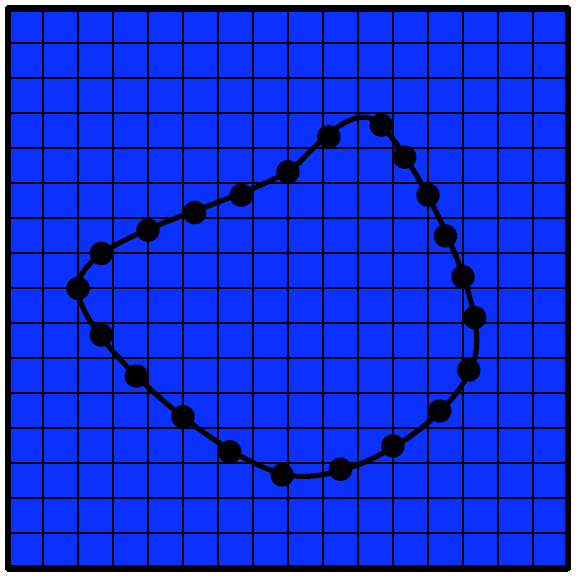
\includegraphics[width=0.78\textwidth]{ch4d-l19-ib-grid.png}
\sourcecredit{Lecture 19, slide 32: the Lagrangian points of a closed boundary on the Eulerian grid.}
\end{columns}
\sourcecredit{Lecture 19, slides 30--32 (the speaker notes: ``now let's move to what we can call numerical experiments'').}
\end{frame}

\begin{frame}{The rules of thumb}
\label{fr:rules}
\footnotesize
\begin{itemize}
  \item Typically you want \al{2 boundary points for every fluid grid point}: $\Delta s = \Delta x/2$. (Fewer, and fluid can pass between the points; IB2d's driver assumes this spacing when it spreads forces, slide \ref{fr:kscaling}.)
  \item \al{Second order in space} if the boundaries are smooth, \al{first order} if there are edges; and first order at the boundary itself, where the regularised delta function smooths everything over 3--4 cells.
  \item For publication-quality results, typically $256 \times 256$ or $512 \times 512$ grids for the fluid domain (2D).
  \item The time step is \al{first or second order}, depending on the version (the lab's time-step study could not measure it: slide \ref{fr:dttab}).
  \item Typically $\Delta t = 10^{-5}$ or $10^{-6}$ when the characteristic time is $t = 1$ and the grid is $512 \times 512$: for example, one wing stroke every 1 unit of time.
\end{itemize}
\begin{punchbox}
\footnotesize What this chapter adds to the list, from the runs: (1) the time step a band tolerates falls with its stiffness, between $k^{-1/2}$ and $1/k$ here (a factor 1.3--4 for ten times the stiffness from the shipped band up, at least 8 from the ten-times-softer band to it); (2) in IB2d a spring constant is a force density and the driver weights it with $L_x/(2N_x)$, so refining the grid with the same $k$ makes a \emph{softer} band: scale $k$ with $N^2$ to keep the physics (and with the number of points when you add points to a grid); (3) a closed band loses enclosed area at a rate set by the grid, not by the points per cell (13\,\% by $t = 1$ at $32^2$, 4\,\% at $256^2$): the standard IB method is not volume-conserving, and conserved quantities are the cheapest convergence check.
\end{punchbox}
\sourcecredit{Lecture 19, slide 33; Lecture 12, slide 21.}
\end{frame}

\begin{frame}[fragile]{The lab's example: the shipped rubber band, as it is}
\label{fr:labband}
\vspace{-1.5mm}
\begin{columns}[T]
\column{0.5\textwidth}
\scriptsize
\code{pyIB2d/Examples/Rubberband\_with\_Springs} (chapter 4a), which is also \code{matIB2d/Examples/}\allowbreak\code{Example\_Standard\_Rubberband/}\allowbreak\code{Rubberband\_with\_Springs} (the course's \code{Rubberband\_HW5} sat in the same folder, with its own generator: slide \ref{fr:blowup2}):
\begin{itemize}
  \item a $1 \times 1$ periodic box, $32 \times 32$ cells, $\mu = 0.01$, $\rho = 1$, $\Delta t = 10^{-3}$, $T = 1.5$, a dump every 20 steps;
  \item 64 points on an ellipse centred at $(0.5, 0.5)$; the generator is called with $(a, b) = (0.4, 0.2)$ but its function takes \code{(N, rmin, rmax)}, so the 0.4 semi-axis is along $y$: the band is \al{tall}, not wide;
  \item springs between neighbours, $k = 2.5 \cdot 10^4$, resting length $0$: the band wants to shrink; the fluid inside (incompressible) stops it, so it should settle to the circle of the same area, $r = \sqrt{0.08} = 0.283$;
  \item the perimeter is 1.94, so $\Delta s = 0.030 = 0.97\,\Delta x$: \al{one point per cell}, although the file says ``2x resolution of the Eulerian grid'' ($N = 2 N_x$ would be two per cell for a perimeter of 1). The driver does not look: its spreading weight is \code{ds = Lx/(2.*Nx)} $= 0.0156$ (line 259 of \code{IBM\_Driver.py}; MATLAB's line 188 takes the smaller of the two directions), two points per cell assumed.
\end{itemize}
\column{0.48\textwidth}
\begin{lstlisting}[style=tiny]
cd pyIB2d/Examples/Stability_Lab
python3 Rubberband.py              # the shipped files, to 1e-16
python3 Rubberband.py 64 1e5       # 64 x 64 grid, k = 1e5
python3 Rubberband.py 32 1e5 0 4   # 32 x 32, two points per cell
python3 main2d.py                  # one run
python3 analyze.py                 # series.csv: shape in time
python3 sweep.py base blowup map   # the chapter's run groups
\end{lstlisting}
\vspace{-2mm}
\scriptsize
\code{examples/IB2d/Stability\_Lab} in the repository: the generator with the grid, stiffness, resting length and points per cell as arguments, the sweep that made every table here (one folder per run under \code{runs/}), and the analysis (centroid, half-extents $r_x$, $r_y$, mean radius, perimeter, enclosed area from the \code{lagsPts} dumps). Dumps are written every 0.02 time units whatever $\Delta t$ is (every step when $\Delta t > 0.02$), each one step late (slide \ref{fr:blowup1py}), so runs compare dump by dump to within one step.
\end{columns}
\end{frame}

\begin{frame}{What the band does}
\label{fr:bandbase}
\centering
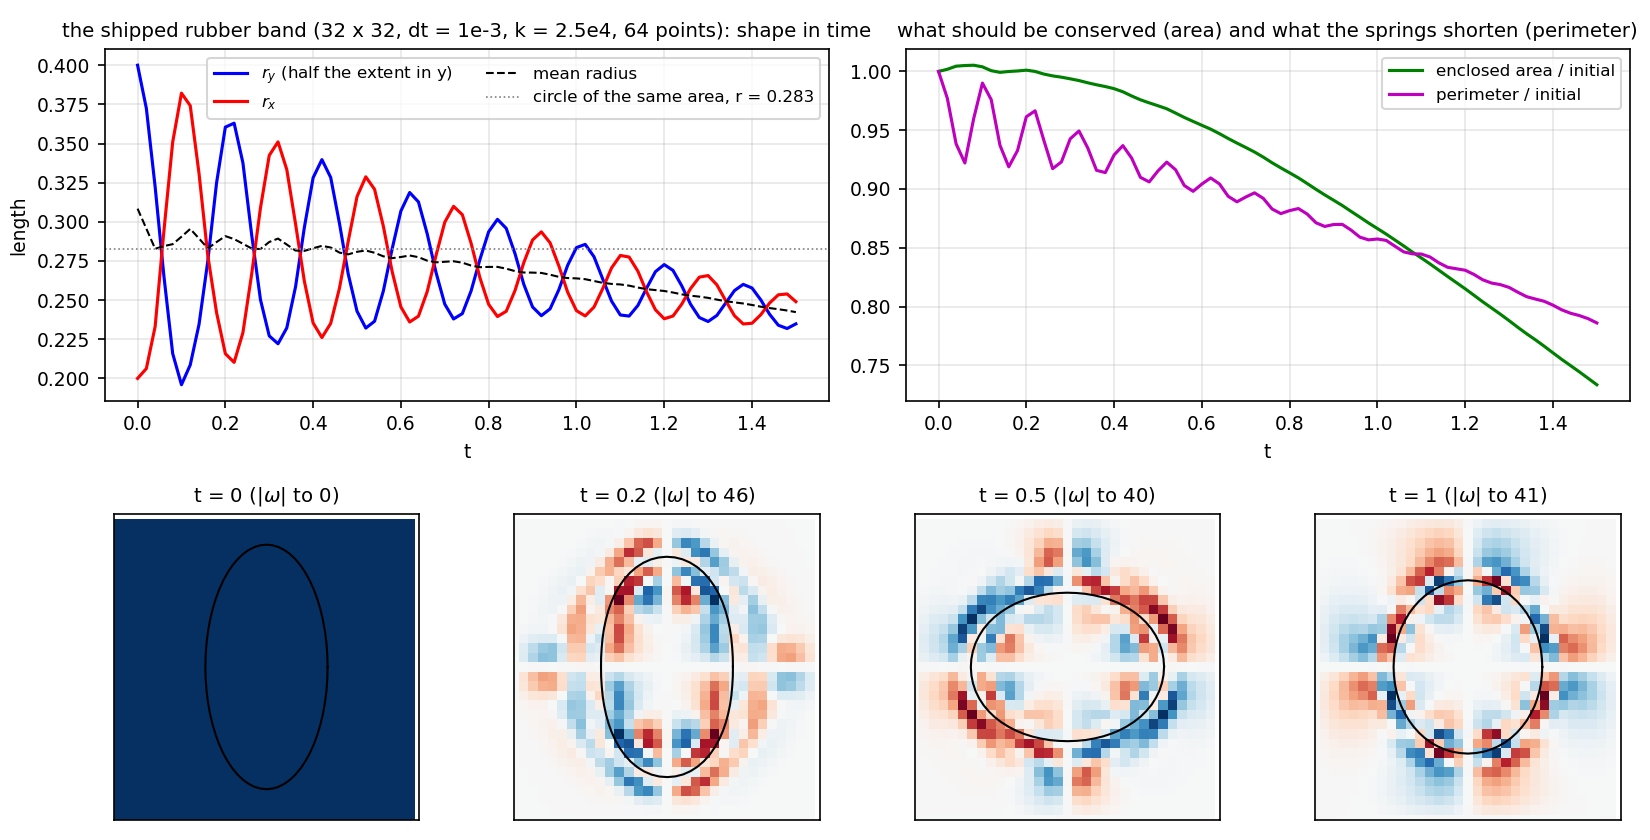
\includegraphics[width=0.72\textwidth]{ch4d-band-base.png}

\footnotesize
The tall ellipse snaps to a wide one and back, seven to eight times in 1.5 units of time (a period of about 0.2: $r_y$ has minima at $t = 0.10, 0.32, 0.52, \ldots, 1.48$), with decaying amplitude ($r_y$ from 0.40 to 0.196 at $t = 0.10$). The mean radius falls below the area-preserving 0.283 because the \al{enclosed area is not conserved}: 97\,\% at $t = 0.5$, 87\,\% at $t = 1$, 73\,\% at $t = 1.5$. The fluid leaks through a band with one point per cell, and the springs (resting length 0) pull the perimeter in by 21\,\%. The four vortices at each ``corner'' are the flow the snapping makes. Run time: 3.7 s for 1500 steps (laptop, Python).
\end{frame}

\begin{frame}[fragile]{Blow-up 1: a time step of 1}
\label{fr:blowup1}
\begin{columns}[T]
\column{0.5\textwidth}
\footnotesize
The course's lab (MATLAB, \code{Rubberband\_HW5}): open \code{input2d}, change \code{dt} to \code{1.0} and \code{Tfinal} to \code{100}, save and run \code{main2d}:
\begin{lstlisting}[style=input]
Temporal_Information {
Tfinal = 100.0            % Final time of simulation (s)
dt = 1.0            % Time-step (s)
}
\end{lstlisting}
\column{0.48\textwidth}
\al{Instability error!}
\begin{lstlisting}[style=tiny]
Error using please_Move_Lagrangian_Point_Positions (line 84)
BLOW UP! (*forces TOO large*) -> try decreasing the time-step
or decreasing material property Stiffnesses
\end{lstlisting}
(In the 2024 code the message comes from lines 95 and 109 of that file: a \code{try}/\code{catch} around the same index look-up that the Python port does unguarded; a \code{NaN} or \code{Inf} position makes an invalid index, MATLAB throws, and the \code{catch} prints the message.) Then change the temporal information back: \code{Tfinal = 2.0}, \code{dt = 1.0e-3}.
\end{columns}
\sourcecredit{Lecture 19, slides 34--35.}
\end{frame}

\begin{frame}[fragile]{Blow-up 1 in Python}
\label{fr:blowup1py}
\begin{columns}[T]
\column{0.5\textwidth}
\footnotesize
\al{Python} (\code{sweep.py blowup}, case \code{dt1\_T100}): the port has no such check. One thing to know first: the port writes dump $k$ after step $k \cdot$ \code{print\_dump} $+\,1$, one step late (its save test runs on the step counter before the counter is incremented, \code{IBM\_Driver.py} line 834; harmless at $\Delta t = 10^{-3}$, visible here at $\Delta t = 1$). The points are spread over the whole box (each moved by $\Delta t\, u$, then wrapped by the periodic box): dump 1, written after step 2, has $r_x = r_y = 0.50$ and a perimeter of 39; dump 2, after step 3, holds only zeros (positions so large that $x \bmod L_x$ is exactly 0 in floating point); dump 3, after step 4, holds only \code{NaN} (coincident points give $0/0$ in the spring direction, \code{please\_Find\_Lagrangian\_}\allowbreak\code{Forces\_On\_Eulerian\_grid.py} line 539); in step 5 a \code{NaN} position is cast to an index:
\column{0.48\textwidth}
\begin{lstlisting}[style=tiny]
File ".../IBM_Blackbox/Supp.py", line 101, in please_Move_Lagrangian_Point_Positions
    distX = give_Eulerian_Lagrangian_Distance(x[xInds], xL_H_ReSize, Lx)
IndexError: index -9223372036854775808 is out of bounds for axis 0 with size 32
\end{lstlisting}
That number is what \code{int(NaN)} gives. Whenever a Python IB2d run ends with this \code{IndexError}, read it as MATLAB's ``BLOW UP'': the time step is too large for the forces (or the forces are too large for the time step), and the first thing to try is the same: halve $\Delta t$ or soften the stiffness.
\end{columns}
\sourcecredit{\code{runs/dt1\_T100/run.log}; \code{IBM\_Driver.py} line 834.}
\end{frame}

\begin{frame}[fragile]{Blow-up 2: a band 1000 times stiffer}
\label{fr:blowup2}
\begin{columns}[T]
\column{0.5\textwidth}
\scriptsize
The course's lab, with $\Delta t$ back at $10^{-3}$: ``there is an inverse relationship between the force the boundary applies to the fluid and the time step required.'' Open \code{generate\_mesh2d.m}:
\begin{lstlisting}[style=mtiny]
mesh_name = 'rubber_band';          % structure name
kappa_spring = 2.0e3;               % spring constant (Newton)
\end{lstlisting}
Change \code{kappa\_spring} to \code{2.0e6}, save, run \code{generate\_mesh2d}, run \code{main2d}:
\begin{lstlisting}[style=tiny]
Error in IBM_Driver (line 794)
    [xLag_h, yLag_h] = please_Move_Lagrangian_Point_Positions(mu, U, V, xLag, yLag,
    xLag, yLag, x, y, dt/2, grid_Info,0,poroelastic_Yes,poroelastic_info,F_Poro);
\end{lstlisting}
(the same BLOW UP, reported one call higher). Change \code{kappa\_spring} back to \code{2.0e3}, save, run \code{generate\_mesh2d} again.
\column{0.48\textwidth}
\scriptsize
The course's \code{generate\_mesh2d.m} is the IBAMR-style generator of chapter 6 adapted to IB2d (the lines the lecture shows are its, comment for comment; how it converts $\kappa$ into IB2d's per-link constant is not on the slides), and its band is that generator's, not the shipped ellipse: a circle of radius 0.1 (with, if the geometry lines were kept, springs at their resting length and a small stretch in $x$), which is what the VisIt picture of slide \ref{fr:visit64} shows. The shipped IB2d band uses \code{Rubberband.m} with \code{k\_Spring = 2.5e4} directly, and that is the band of this chapter's lab.
\end{columns}
\sourcecredit{Lecture 19, slide 36.}
\end{frame}

\begin{frame}{Blow-up 2 in Python, and what the two blow-ups look like}
\label{fr:blowup2py}
\centering
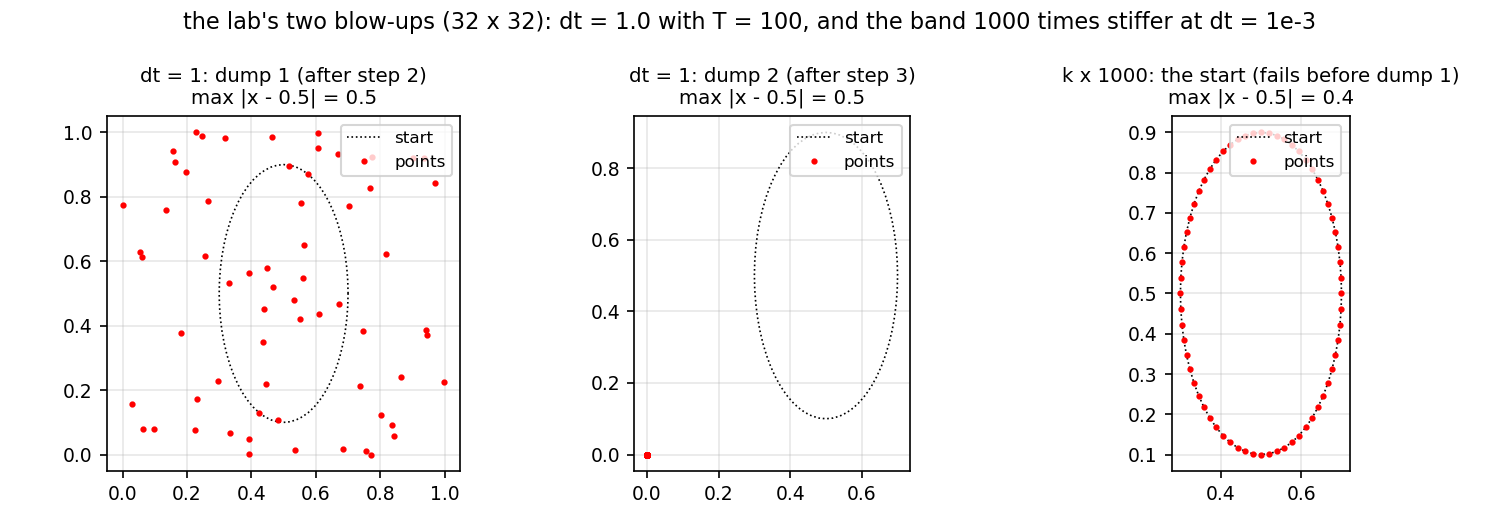
\includegraphics[width=0.8\textwidth]{ch4d-band-blowup.png}

\footnotesize
Python: \code{python3 Rubberband.py 32 2.5e7} then \code{main2d.py} (case \code{k1000x}): the same \code{IndexError} before the first dump (step 21 at this $\Delta t$), and the run takes no longer than the port's start-up (1.3 s, against 1.5 s plus 1.2 ms per step for the runs that live), so within the first few steps; not one dump beyond the initial one. Both blow-ups take a second of computing.
\end{frame}

\begin{frame}{The inverse relationship, measured: 41 runs}
\label{fr:map}
\centering
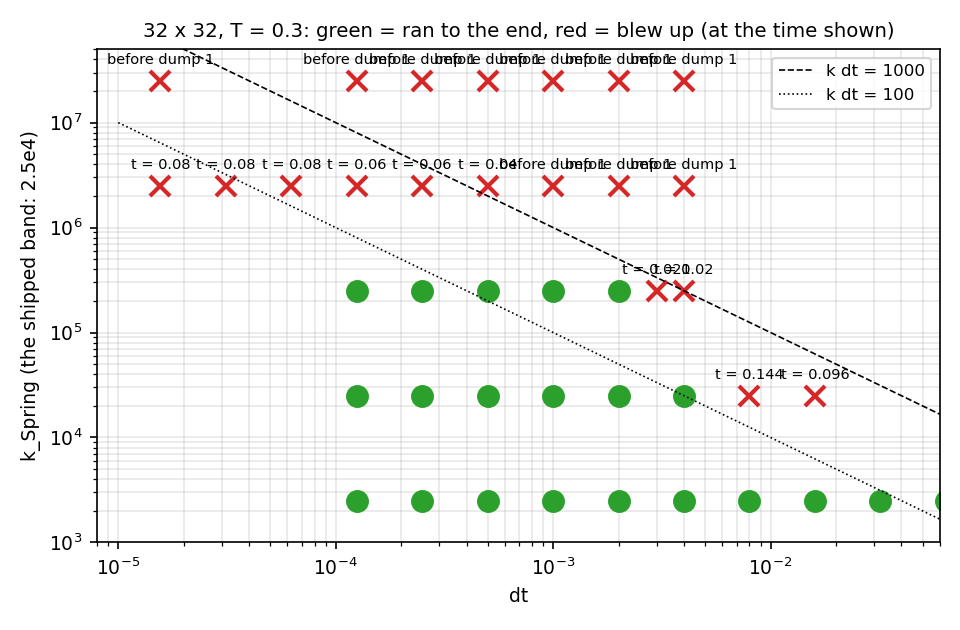
\includegraphics[width=0.63\textwidth]{ch4d-band-map.png}

\footnotesize
Stiffness $\times$ time step on the $32^2$ grid, each run to $T = 0.3$ (\code{sweep.py map map2}). Green: ran to the end. Red: the \code{IndexError}, at the time of the last dump written (``step 1'' in the figure means that no dump beyond the first was written, i.e. failure before $t = 0.02$; slide \ref{fr:mapnum} says how early). The dotted and dashed lines are $k\,\Delta t = 100$ and $1000$.
\end{frame}

\begin{frame}{The map as numbers}
\label{fr:mapnum}
\scriptsize
\begin{tabular}{@{}L{0.08\textwidth}L{0.13\textwidth}L{0.15\textwidth}L{0.38\textwidth}L{0.1\textwidth}@{}}
\toprule
$k$ & relative to the shipped band & survives up to $\Delta t$ & fails at & $k\,\Delta t$ at the edge \\
\midrule
$2.5 \cdot 10^3$ & $\times 0.1$ & 0.064 (every value tried) & -- & $> 160$ \\
$2.5 \cdot 10^4$ & $\times 1$ & 0.004 & 0.008 ($t = 0.14$), 0.016 ($t = 0.10$) & 100--200 \\
$2.5 \cdot 10^5$ & $\times 10$ & 0.002 & 0.003 and 0.004 ($t = 0.02$) & 500--750 \\
$2.5 \cdot 10^6$ & $\times 100$ & none & before the first dump ($t < 0.02$) at $\Delta t = 0.004$, $0.002$, $0.001$; $t = 0.04$ at $5 \cdot 10^{-4}$, $0.06$ at $2.5$ and $1.25 \cdot 10^{-4}$, $0.08$ at $6.25 \cdot 10^{-5}$ down to $1.6 \cdot 10^{-5}$ & -- \\
$2.5 \cdot 10^7$ & $\times 1000$ & none & before the first dump ($t < 0.02$) for every $\Delta t$: within the first few steps for $\Delta t \ge 1.25 \cdot 10^{-4}$ (wall time = start-up), after some 1100 steps at $1.6 \cdot 10^{-5}$ (1.4 s of stepping) & -- \\
\bottomrule
\end{tabular}

\footnotesize
Read along a row: the shipped band takes a step of 0.004 and not 0.008; ten times stiffer, 0.002 and not 0.003. Read down a column: at $\Delta t = 10^{-3}$ the band may be ten times stiffer than shipped, not a hundred. The run time to $T = 0.3$ at $32^2$ is 1.4--4.5 s whatever happens (6 and 10 s for the two smallest steps, $3 \cdot 10^{-5}$ and $1.6 \cdot 10^{-5}$), so a map like this costs minutes, and it is the cheapest way to know where an example of your own stands.
\end{frame}

\begin{frame}{Reading the map}
\label{fr:mapread}
\scriptsize
\begin{itemize}
  \item The lecture's statement holds in direction: the stiffer the band, the smaller the admissible step. The exponent is not clean. From the shipped band to the one ten times stiffer, $\Delta t_{\max}$ falls by a factor between 1.3 and 4 (the edges lie in $[0.004, 0.008)$ and $[0.002, 0.003)$), closer to $k^{-1/2}$, the scaling of a mass--spring system ($\Delta t < 2/\omega$, $\omega = \sqrt{k/m}$) with the fluid as the mass, than to $1/k$; from the band ten times softer to the shipped one it falls by at least 8--16 (0.064, the largest step tried, still ran at $k \times 0.1$), which is $1/k$ or steeper. At the edge, $k\,\Delta t$ is $> 160$, 100--200 and 500--750: of order $10^2$--$10^3$, not a constant.
  \item The band 100 times stiffer is a different story: for every $\Delta t$ from $5 \cdot 10^{-4}$ down to $1.6 \cdot 10^{-5}$ it fails at nearly the same moment (between $t = 0.04$ and $0.10$, later for the smaller steps), and for $\Delta t \ge 10^{-3}$ before the first dump. Its dumps up to then are not the fast snap a band a hundred times stiffer should show (ten times the speed of the shipped band, by the $T^{-1/2}$ scaling of slide \ref{fr:kscaling}): $r_y$ falls only from 0.40 to 0.29 by $t = 0.08$, slower than the shipped band's 0.22, while the perimeter is already 11\,\% and the enclosed area 7\,\% down. A smaller step does not save it, so the step is not what limits it; whether a finer grid does, which would say the failure is the grid's (the fluid at those speeds on 32 cells), is exercise 6 of slide \ref{fr:exercises}.
  \item The band 1000 times stiffer fails before its first dump at every $\Delta t$ tried, down to $1.6 \cdot 10^{-5}$: within the first few steps for $\Delta t \ge 1.25 \cdot 10^{-4}$ (the run takes no longer than the start-up), after some 1100 steps at $1.6 \cdot 10^{-5}$ (1.4 s of stepping at 1.2 ms per step). With resting length 0 the tension in each of its links is $k\,\Delta s \approx 7.5 \cdot 10^5$ (the net force on a point is the difference of its two links' pulls), and a step short enough to live with it was not found.
  \item Lecture 12's strategy stands: avoid large forces (large accelerations, very stiff springs); a stiff band costs time steps as well as steps.
\end{itemize}
\end{frame}

\begin{frame}[fragile]{Refining the grid, the course's way}
\label{fr:refinecourse}
\begin{columns}[T]
\column{0.5\textwidth}
\footnotesize
\code{generate\_mesh2d.m}:
\begin{lstlisting}[style=mtiny]
L = 1;                              % length of computational domain (m)
N = 32;                             % number of Cartesian grid meshwidths at the finest level of the AMR grid
dx = L/N;                           % Cartesian mesh width (m)
\end{lstlisting}
``This is a pretty coarse simulation since there are only 32 spatial grid points in each direction. Let's change it to 64.'' Change \code{N} to \code{64}.
\begin{lstlisting}[style=mtiny]
npts = ceil(2*(band_length/L)*N);   % number of points along the rubber band
ds = band_length/(npts);            % physical distance between neighboring Lagrangian mesh points (m)
\end{lstlisting}
``This will set \code{ds} to approximately \code{dx/2}.'' Run the code to generate new files.
\column{0.48\textwidth}
\footnotesize
\code{input2d}: ``you also need to update the grid size.''
\begin{lstlisting}[style=input]
Grid_Parameters {
Nx = 32                % # of Eulerian Grid Pts. in x-Direction (MUST BE EVEN!!!)
Ny = 32                % # of Eulerian Grid Pts. in y-Direction (MUST BE EVEN!!!)
\end{lstlisting}
Change \code{Nx} and \code{Ny} to \code{64}, save and run \code{main2d}.
\begin{punchbox}
\small Two files must agree: the generator's grid (it sets $\Delta s$ from $\Delta x$) and \code{input2d}'s. The shipped generators say so in capitals (``MAKE SURE MATCHES IN input2d''), and nothing checks it: a band generated for 64 and run on 32 has four points per cell and a different stiffness per unit length. The lab's \code{sweep.py} writes both from one number.
\end{punchbox}
\end{columns}
\sourcecredit{Lecture 19, slides 38--39.}
\end{frame}

\begin{frame}{What refinement does to the band in IB2d}
\label{fr:kscaling}
\footnotesize
IB2d spreads each point's force to the grid as a line integral, $f(x) = \sum_i F_i\, \delta_h(x - X_i)\, \Delta s$ (\code{Fx = ((fx*ds) * delta\_Y) @ delta\_X}), with \al{the driver's own $\Delta s = L_x/(2N_x) = \Delta x/2$}, not the spacing of your file. Each spring's force is $k(|d| - L)$ with $|d| \approx \Delta s_{\text{file}}$ when $L = 0$, so one link gives the fluid $k\,\Delta s_{\text{file}}\,\Delta x/2$, and the band's effective tension is $T \propto k\,\Delta s_{\text{file}}\,\Delta x$. Two consequences:
\begin{itemize}
  \item \al{refining the grid} ($\Delta s_{\text{file}} \propto \Delta x$, as the generators do) with the same $k$ makes the band \al{four times softer} per doubling: keep $k\,\Delta x^2$, i.e. scale $k$ with $N^2$;
  \item \al{adding points on the same grid} with the same $k$ halves the tension: scale $k$ with the number of points.
\end{itemize}
\vspace{-2mm}
\begin{center}
\tiny
\begin{tabular}{@{}llllll@{}}
\toprule
what was changed & $k$ & $T$ (shipped band = 1) & first $r_y$ minimum at & period & \\
\midrule
$64^2$, same file $k$ (the naive refinement) & $2.5 \cdot 10^4$ & $1/4$ & $t = 0.20$ & $\times 2$ & softer still \\
$64^2$, $k \propto N$ (``keep $k\,\Delta s$'') & $5 \cdot 10^4$ & $1/2$ & $t = 0.14$ & $\times 1.4$ & softer \\
$64^2$, $k \propto N^2$ & $10^5$ & 1 & $t = 0.10$ & $\times 1$ & the same band \\
$32^2$, twice the points, $k \times 4$ & $10^5$ & 2 & $t = 0.06$--$0.08$ & $\times 0.7$ & stiffer \\
$32^2$, twice the points, $k \times 2$ & $5 \cdot 10^4$ & 1 & $t = 0.10$ & $\times 1$ & the same band \\
\bottomrule
\end{tabular}
\end{center}
The oscillation period is the check: it scales as $T^{-1/2}$, like a mass on a spring; only the rows with $T = 1$ keep the first minimum at $t = 0.10$, on every grid from $32^2$ to $256^2$ (next slide). Which row the course's recipe is depends on a line the lecture does not show: if its \code{generate\_mesh2d.m} kept the IBAMR original's $\kappa\,\Delta s/\Delta s^2$, the file constant doubles when $\Delta s$ halves and the recipe is the $k \propto N$ row. The IBAMR convention differs (chapter 6: the file's spring constant is $K/\Delta s$, a tension per unit strain divided by the spacing, which the generators write as $\kappa\,\Delta s/\Delta s^2$); whichever code, decide what must stay fixed under refinement and write the generator so that it does.
\end{frame}

\begin{frame}{Refining with the band kept: $16^2$ to $256^2$}
\label{fr:gridfig}
\centering
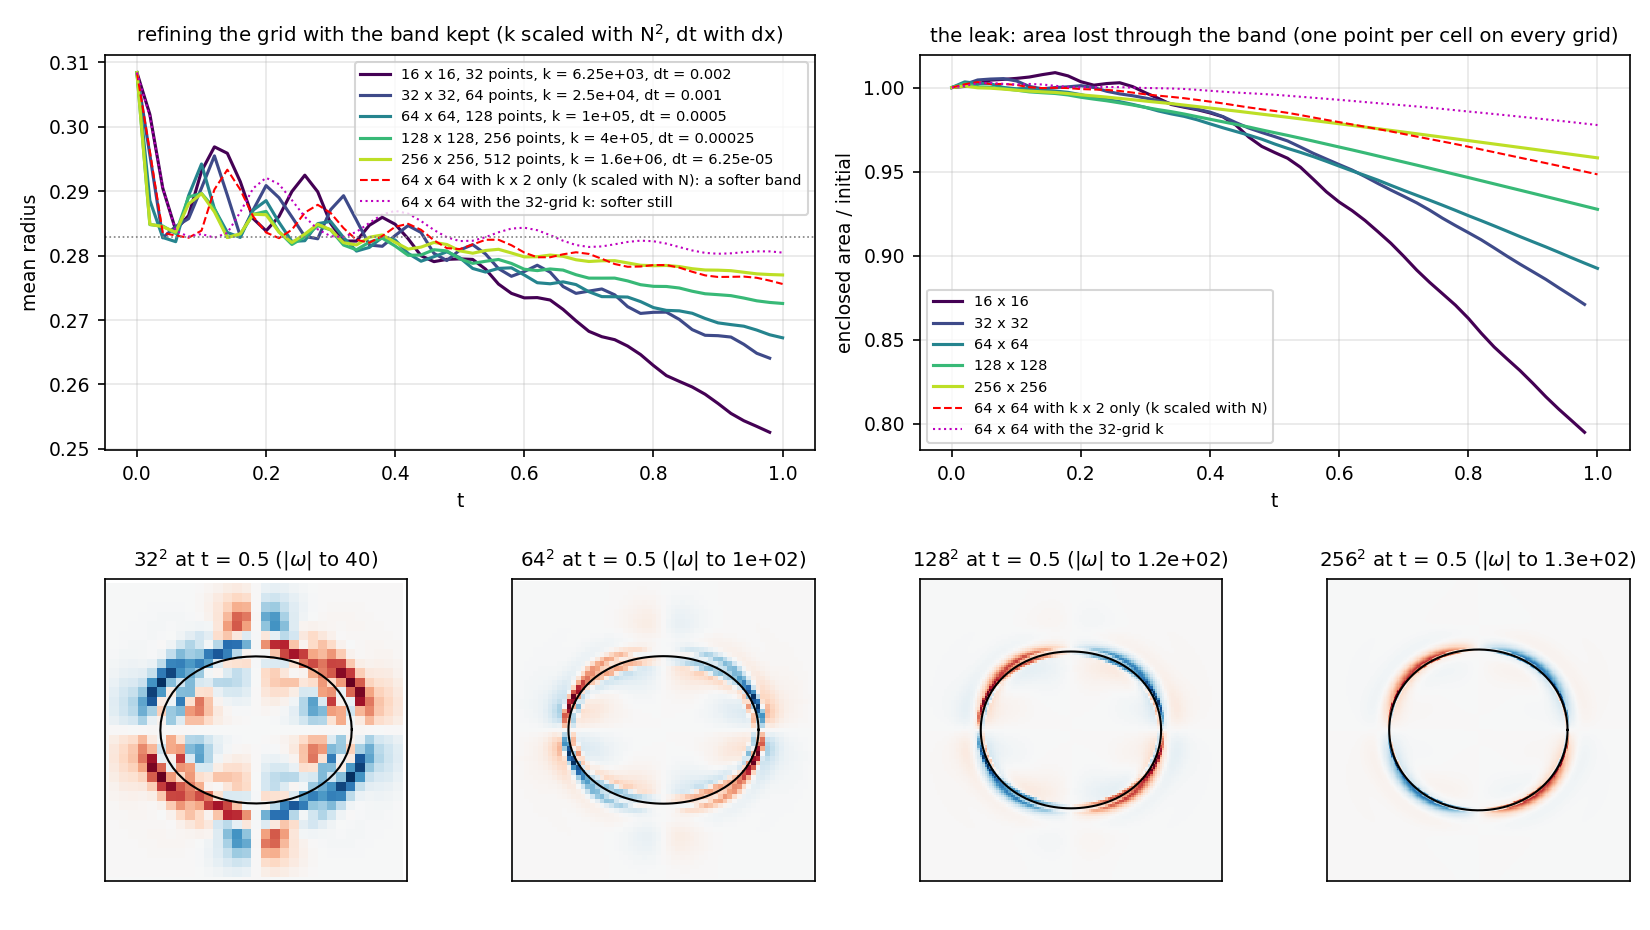
\includegraphics[width=0.81\textwidth]{ch4d-band-grid.png}
\sourcecredit{\code{sweep.py grid2} (solid: $k = 2.5 \cdot 10^4\,(N/32)^2$, $\Delta t = 10^{-3} \cdot 32/N$, halved again at $256^2$); the dashed and dotted $64^2$ runs are the two wrong refinements of the previous slide.}
\end{frame}

\begin{frame}{The numbers at $t = 0.98$, and the leak}
\label{fr:gridtab}
\begin{columns}[T]
\column{0.6\textwidth}
\tiny
\begin{tabular}{@{}rrrrrrr@{}}
\toprule
grid & points & $k$ & $\Delta t$ & first $r_y$ min & area left & wall \\
\midrule
$16^2$ & 32 & $6.25 \cdot 10^3$ & $2 \cdot 10^{-3}$ & 0.200 at 0.12 & 79.5\,\% & 1.9 s \\
$32^2$ & 64 & $2.5 \cdot 10^4$ & $10^{-3}$ & 0.196 at 0.10 & 87.1\,\% & 2.9 s \\
$64^2$ & 128 & $10^5$ & $5 \cdot 10^{-4}$ & 0.203 at 0.10 & 89.6\,\% & 8.6 s \\
$128^2$ & 256 & $4 \cdot 10^5$ & $2.5 \cdot 10^{-4}$ & 0.201 at 0.10 & 93.0\,\% & 38 s \\
$256^2$ & 512 & $1.6 \cdot 10^6$ & $6.25 \cdot 10^{-5}$ & 0.203 at 0.10 & 95.9\,\% & 384 s \\
\bottomrule
\end{tabular}

\footnotesize
mean radius at $t = 0.98$: 0.2526, 0.2641, 0.2677, 0.2727, 0.2771, climbing towards the area-preserving 0.283 as the leak closes; successive differences 0.0115, 0.0036, 0.0050, 0.0043.
\column{0.38\textwidth}
\scriptsize
\begin{itemize}
  \item The band's \al{dynamics} are converged from $32^2$ on: the first minimum (depth 0.196--0.203, time 0.10) agrees to 2\,\% on every grid from $32^2$ on ($16^2$ is late, at $t = 0.12$).
  \item Its \al{area} is not: 4--20\,\% of the enclosed fluid is gone by $t = 1$, and the loss falls only slowly with resolution (by a fifth to two fifths per doubling, 20.5, 12.9, 10.4, 7.0, 4.1\,\%: an order between 0.3 and 0.8). That is why $r_y$ and the mean radius at a fixed late time do not line up as a clean $p$: the leak, not the discretisation of the dynamics, dominates the late-time numbers.
  \item Two points per cell do not change it (next slide): it is the method's volume error, which only the grid reduces.
\end{itemize}
\end{columns}
\end{frame}

\begin{frame}{Two points per cell: the same band, the same area loss}
\label{fr:ppc}
\centering
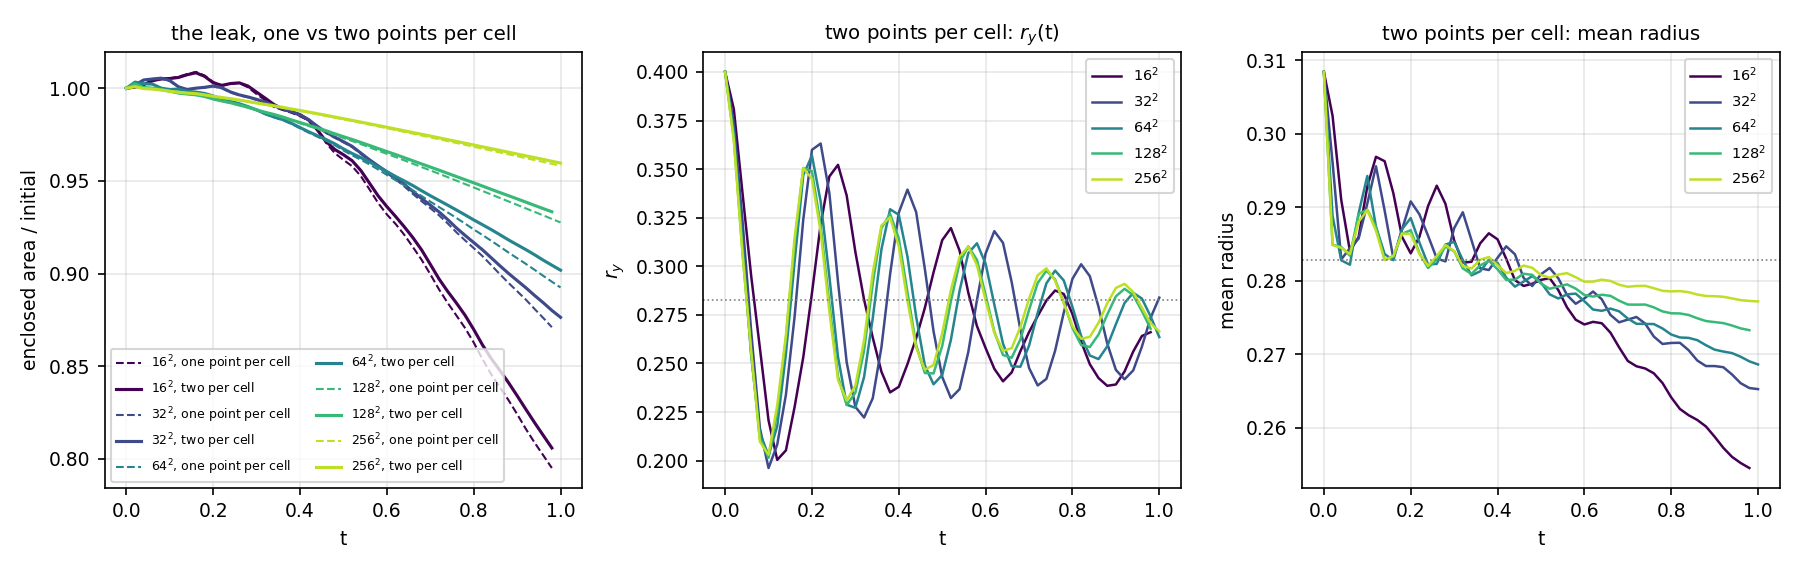
\includegraphics[width=0.88\textwidth]{ch4d-band-ppc.png}

\scriptsize
\begin{tabular}{@{}rrrrrr@{}}
\toprule
grid & points & $k$ & area left at $t = 0.98$ & same, one point per cell & first $r_y$ min \\
\midrule
$16^2$ & 64 & $1.25 \cdot 10^4$ & 80.6\,\% & 79.5\,\% & 0.200 at 0.12 \\
$32^2$ & 128 & $5 \cdot 10^4$ & 88.0\,\% & 87.1\,\% & 0.196 at 0.10 \\
$64^2$ & 256 & $2 \cdot 10^5$ & 90.5\,\% & 89.6\,\% & 0.203 at 0.10 \\
$128^2$ & 512 & $8 \cdot 10^5$ & 93.3\,\% & 93.0\,\% & 0.202 at 0.10 \\
$256^2$ & 1024 & $3.2 \cdot 10^6$ & 96.1\,\% & 95.9\,\% & 0.203 at 0.10 \\
\bottomrule
\end{tabular}
\sourcecredit{\code{sweep.py grid4}: twice the points on every grid, $k$ doubled with them (slide \ref{fr:kscaling}), $\Delta t$ halved (except at $256^2$, where both series use $6.25 \cdot 10^{-5}$); dashed: the one-point-per-cell series of slide \ref{fr:gridtab}.}
\end{frame}

\begin{frame}{What the two-point series says}
\label{fr:ppc2}
\small
\code{sweep.py grid4}: twice the points on every grid, $k$ doubled with them (slide \ref{fr:kscaling}), $\Delta t$ halved (except at $256^2$, where both series use $6.25 \cdot 10^{-5}$). It is the same band (first minimum 0.196--0.203 at $t = 0.10$ from $32^2$ on), and it loses \al{the same area} as the one-point-per-cell band, to within one percent on every grid.

So the loss is not fluid passing between points. It is the standard IB method's \al{volume error} (Peskin and Printz 1993): the velocity interpolated to the points is not exactly divergence-free along the boundary, so a closed boundary gains or loses area at a rate set by the grid: 20, 13, 10, 7, 4\,\% at $t = 1$ from $16^2$ to $256^2$, an order between 0.3 and 0.8, unevenly.

Remedies: refine; a volume-conserving variant (Peskin--Printz's modified divergence; IBAMR's staggered-grid scheme does better: B.\,E. Griffith, ``On the volume conservation of the immersed boundary method'', Commun.\ Comput.\ Phys.\ 12 (2012) 401--432; chapter 5 describes the scheme); or measure what does not depend on the enclosed area. The two-points-per-cell rule still holds for what it is for: a boundary that must not let fluid \emph{through} it (a wall with target points, chapter 4c).
\end{frame}

\begin{frame}{The time step, at $64^2$}
\label{fr:dttab}
\centering
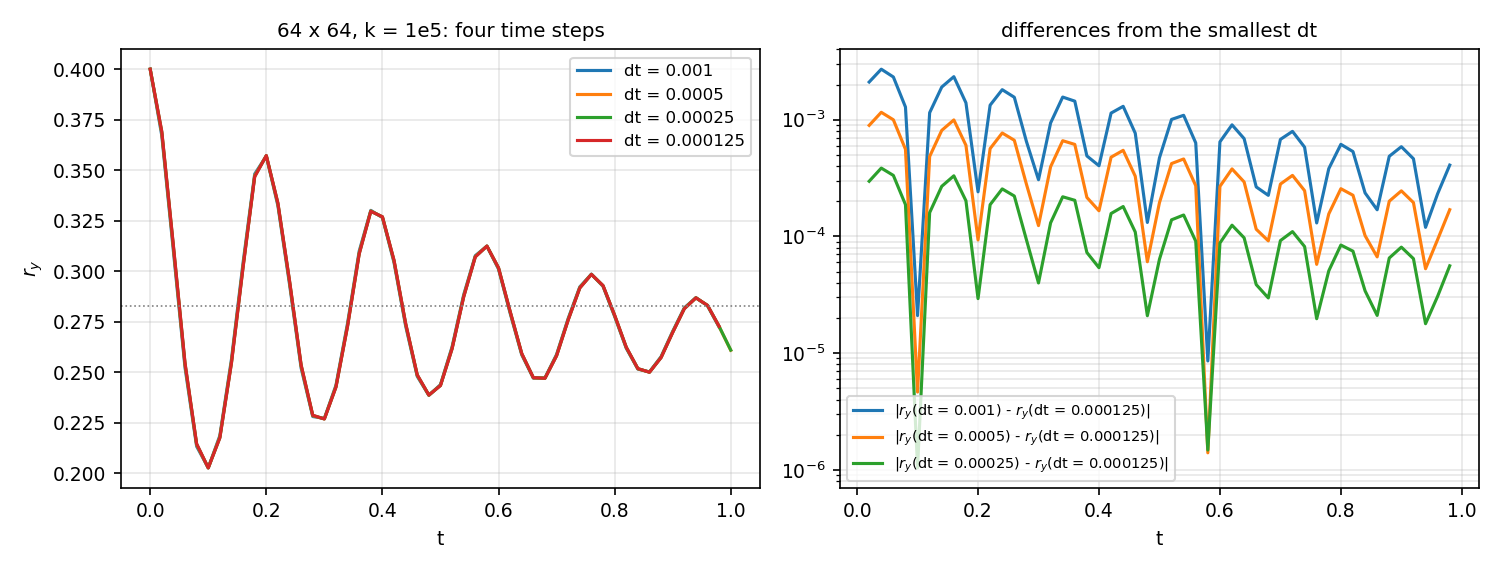
\includegraphics[width=0.76\textwidth]{ch4d-band-dt.png}

\scriptsize
\begin{tabular}{@{}lllllll@{}}
\toprule
$\Delta t$ & $10^{-3}$ & $5 \cdot 10^{-4}$ & $2.5 \cdot 10^{-4}$ & $1.25 \cdot 10^{-4}$ & differences of $r_y(0.98)$ & $p$ \\
\midrule
$r_y$ at $t = 0.98$ & 0.272311 & 0.272550 & 0.272664 & 0.272719 & $2.4 \cdot 10^{-4}$, $1.1 \cdot 10^{-4}$, $5.6 \cdot 10^{-5}$ & 1.07, 1.02 \\
wall & 5.8 s & 8.5 s & 14.3 s & 23.4 s & & \\
\bottomrule
\end{tabular}
\sourcecredit{\code{sweep.py dt2}: $64^2$, $k = 10^5$, $T = 1$. Halving $\Delta t$ halves the difference, which looks like \al{first order}; but it is the dumps' lag, not the time stepping. The port writes every dump one step late (slide \ref{fr:blowup1py}), so dump 49 of the $\Delta t = 10^{-3}$ run is the state at $t = 0.981$ and of the $1.25 \cdot 10^{-4}$ run at $0.98013$; with $r_y$ falling at 0.52 per unit time there, the lag alone accounts for $4.5 \cdot 10^{-4}$, $1.9 \cdot 10^{-4}$ and $6.5 \cdot 10^{-5}$ of the $4.1 \cdot 10^{-4}$, $1.7 \cdot 10^{-4}$ and $5.6 \cdot 10^{-5}$ measured against the finest run, and the differences change sign with the slope of $r_y$ ($+5.9 \cdot 10^{-4}$ at $t = 0.90$, where $r_y$ rises). What the four runs do show is that the time-stepping error is below the lag, under $10^{-4}$ in $r_y$ at $\Delta t = 10^{-3}$; its order is not measured here (exercise 7). The four curves are indistinguishable on the left; the largest step is $10^{-3}$ of $r_y$ away from the smallest.}
\end{frame}

\begin{frame}{What refinement costs}
\label{fr:cost}
\footnotesize
\begin{center}
\scriptsize
\begin{tabular}{@{}lrrrrr@{}}
\toprule
grid & $32^2$ & $64^2$ & $128^2$ & $256^2$ & \\
\midrule
cells & 1024 & 4096 & 16384 & 65536 & $\times 4$ \\
points & 64 & 128 & 256 & 512 & $\times 2$ \\
steps to $t = 1$ ($\Delta t \propto \Delta x$) & 1000 & 2000 & 4000 & 16000 & $\times 2$ (and $\times 4$ at $256^2$) \\
wall (Python, laptop) & 2.9 s & 8.6 s & 38 s & 384 s & $\times 3$--$10$ \\
per step & 2.9 ms & 4.3 ms & 9.5 ms & 24 ms & \\
\bottomrule
\end{tabular}
\end{center}
\begin{itemize}
  \item Each doubling of the grid costs $4\times$ the cells, $2\times$ the points and $2\times$ the steps: $16\times$ in the limit, $8\times$ in 2D when the fluid solve dominates. The $512^2$ of the rules of thumb at $\Delta t = 10^{-5}$ is $10^5$ steps per unit time: hours in MATLAB, a cluster job in Python as shipped.
  \item The Python port spreads forces by a dense delta-matrix product: two matrices of $N_b \times N_x$ and $N_y \times N_b$ ($512 \times 256$ at $256^2$), multiplied through every cell of the grid, $O(N_x N_y N_b)$ per step for a kernel that touches 16 cells per point; the fork branch \code{python-updates-2026} (pull request 34 to IB2d, October 2026) replaces it with the local four-point stencil, $O(16 N_b)$: the same numbers (the shipped band's dumps agree to $10^{-10}$), $1.4\times$ faster on the $32^2$ band, and a spreading cost that no longer grows with the number of cells.
  \item The time step shrank with $\Delta x$ here because the stiffness grew with $1/\Delta s^2$ (slide \ref{fr:kscaling}) and, if $\Delta t_{\max}$ falls as $k^{-1/2}$ (slide \ref{fr:mapread}), refining the grid with the same band halves the admissible step as well; the series ran at $\Delta t \propto \Delta x$ throughout, and exercise 5 measures whether that is the limit. That is the second half of ``$\Delta t = 10^{-5}$ at $512^2$''.
\end{itemize}
\end{frame}

\begin{frame}{What the course saw in VisIt}
\label{fr:visit64}
\begin{columns}[T]
\column{0.5\textwidth}
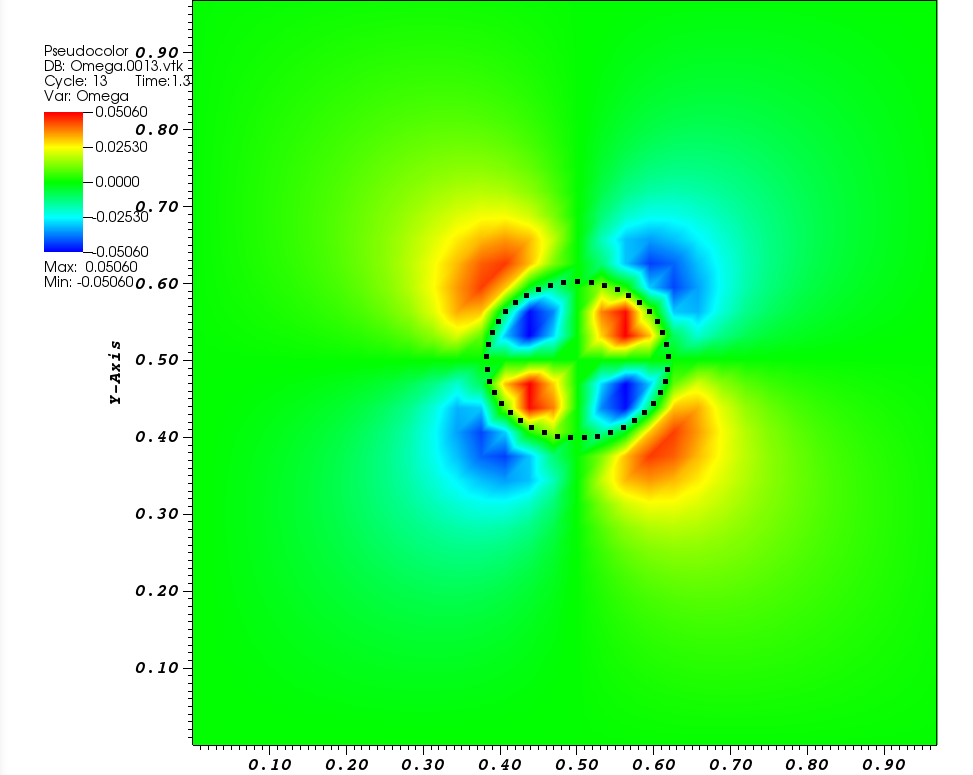
\includegraphics[width=0.88\textwidth]{ch4d-l19-visit-omega.png}
\sourcecredit{Lecture 19, slide 37 (before the refinement slides 38--39): VisIt, Pseudocolor of \code{Omega} from \code{Omega.0013.vtk}, cycle 13, the MATLAB writer's stamp \code{Time: 1.3} (so the course's \code{input2d} dumped every 0.1 time units), automatic colour limits $\pm 0.0506$, the band as about 40 dots on a circle of radius 0.1.}
\column{0.48\textwidth}
\scriptsize
The homework's picture: the course's band with its four vortex pairs, the same quadrupole pattern as the panels of slide \ref{fr:bandbase}, but a different band. The dots lie on a circle of radius 0.1 about $(0.5, 0.5)$, about 40 of them (the IBAMR-style generator gives 41 points at $N = 32$ and 81 at 64, so this is the $32^2$ run), and the vorticity is $0.05$ against our 40: that is the IBAMR-style band of chapter 6 with $\kappa = 2 \cdot 10^3$ (a circle of radius 0.1 which, if the course's copy kept the original's geometry lines, starts from a small stretch with its springs at their resting length and relaxes), not the shipped ellipse with resting length 0 that snaps from tall to wide.
\end{columns}
\end{frame}

\begin{frame}{Comparing two resolutions in VisIt}
\label{fr:visit64b}
\small
What to compare between two resolutions in VisIt (chapter 4b): the same cycle is \emph{not} the same time when $\Delta t$ changed (use the dump interval in time units: here a dump every 0.02); the colour limits must be set by hand to the same values; the band's \code{lagsPts} overlaid on \code{Omega} shows where the vorticity sits relative to the points, which is where a leak would show as flow through the band.
\end{frame}

\begin{frame}{A protocol for an example of your own}
\label{fr:protocol}
\small
\begin{enumerate}
  \item \al{Decide what must stay fixed under refinement} (tension, bending stiffness, target stiffness per unit length) and write the generator so that $k$ follows $\Delta s$ accordingly (slide \ref{fr:kscaling}); make the generator and \code{input2d} take the grid from one number.
  \item \al{Points at $\Delta x/2$} along every boundary that must not leak; check $\Delta s/\Delta x$ printed by the generator, not assumed from a comment.
  \item \al{Find the time step}: start from a working example's $\Delta t$; if the run ends in \code{BLOW UP} or the \code{IndexError}, halve $\Delta t$ (and, if it still fails at a tenth, suspect the forces or the grid, not the step: slide \ref{fr:mapread}); then halve it once more and check that a number you care about moves by less than you care about (slide \ref{fr:dttab}).
  \item \al{Refine the grid once} with the band kept ($k$ rescaled, $\Delta t$ rescaled with $\Delta x$) and compare the same number at the same times: the dumps must land on the same times (set \code{print\_dump} from $\Delta t$).
  \item \al{Report three resolutions}, not two, before quoting an order (slide \ref{fr:sixth}); report the one that converged and what it cost.
  \item \al{Conserved quantities are the cheapest check}: the area inside a closed band, the mass of a tracer, the total circulation; a leak shows there long before it shows in a picture.
\end{enumerate}
\end{frame}

\begin{frame}{Exercises}
\label{fr:exercises}
\small
\begin{enumerate}
  \item The course's homework 5, part 1: run \code{stiff\_ode\_example} with $(0.2, 1)$, $(0.1, 1)$, $(0.01, 1)$ and explain each plot with the factor $1 - 15\Delta t$; then add the trapezoidal step (slide \ref{fr:trap}) and repeat.
  \item Part 2: \code{heat\_equation} with $T = 100$ and $n = 3, 5, 10, 20$, then $n = 10$ and $T = 2, \ldots, 64$; tabulate $r$ and the maximum error; find the $T$ at which $n = 20$ beats $n = 10$, and explain it with slide \ref{fr:sixth}.
  \item Part 3: the rubber band at $\Delta t = 1$ and at 1000 times the stiffness, in MATLAB or Python; quote the exact error line of your port.
  \item Part 4: refine $32 \to 64$ the course's way (same $\kappa$ in \code{generate\_mesh2d.m}, both files updated) and the chapter's way (\code{sweep.py grid2}); compare the time of the first $r_y$ minimum between the two and say which run is ``the same band''.
  \item Extend the map (slide \ref{fr:map}) along a line $k = 2.5 \cdot 10^4$ at $64^2$ and $128^2$: does $\Delta t_{\max}$ halve with $\Delta x$?
  \item The 100-times-stiffer band fails by $t = 0.1$ at every $\Delta t$ on $32^2$ (before the first dump for $\Delta t \ge 10^{-3}$): run it at $64^2$ and $128^2$ with $\Delta t = 10^{-4}$ and report whether a finer grid takes it.
\end{enumerate}
\end{frame}

\begin{frame}{Exercises (2)}
\label{fr:exercises2}
\small
\begin{enumerate}
  \setcounter{enumi}{6}
  \item Measure the order in time of IB2d on the same band ($64^2$, four time steps), in Python or MATLAB (\code{analyze.py} reads the MATLAB dumps too), with the dumps' one-step lag removed (slide \ref{fr:dttab}): compare states at the same step-corrected time, or compare the time of the first minimum of $r_y$ interpolated from the dumps, or use the fork branch's final dump, which is written at exactly $T_{\text{final}}$: first or second?
  \item Run the grid series one grid further ($512^2$, a cluster job: chapter 1) and add the row to the tables of slides \ref{fr:gridtab} and \ref{fr:ppc}.
  \item The volume error: plot the area inside the band against time for $32^2$ to $256^2$ and fit the loss at $t = 1$ to a power of $\Delta x$; then run the same band in IBAMR (chapter 5's rubber band, \code{examples/IB/01-rubber-band}) at the same resolutions and compare.
\end{enumerate}
\end{frame}

\begin{frame}{Preparing the project geometry: the course's homework 6}
\label{fr:hw6}
\small
\al{The course's homework 6 (``you will share your geometry that you will use for your project''):}
\begin{itemize}
  \item 3D print or ANSYS: find a 3D object online (Thingiverse, GrabCAD) and explain what it is, or leave a note of anything you cannot find; create your own (SolidWorks, Autodesk Fusion); or mix: find an object and distort it. Share those objects.
  \item IB2d: geometries are created with a generator (\code{generate\_mesh}, chapter 4c); write code that gives the $x, y$ coordinates of the shape you want and submit it; if the object moves, give pseudo-code for how (the \code{update\_*} functions of chapter 4c).
\end{itemize}
Appendix C collects the homework bank.
\sourcecredit{Lecture 19, slides 2 and 40.}
\end{frame}

\begin{frame}{Summary}
\label{fr:summary}
\footnotesize
\begin{itemize}
  \item Stability is a multiplier: Euler on $y' = -15y$ multiplies by $1 - 15\Delta t$ every step, the explicit heat scheme multiplies the sawtooth mode by $1 - 4r$; outside $|{\cdot}| \le 1$ the run is garbage after a few steps, though it may look fine for a while if the bad mode starts at round-off.
  \item Convergence is measured, with three resolutions and a number you care about; the order says what a refinement buys, and error terms of opposite sign exist ($r = 1/6$).
  \item IB2d blows up the same way whatever the port: MATLAB says \code{BLOW UP}, Python says \code{IndexError: index -9223372036854775808}. Halve $\Delta t$ or soften the force; the admissible step falls with the stiffness (between $k^{-1/2}$ and $1/k$ here), and a band too stiff or too fast for its grid fails at every $\Delta t$.
  \item A spring constant in IB2d is a force density: keep $k\,\Delta s\,\Delta x$ fixed when you refine ($k\,\Delta x^2$ when the points follow the grid, $k \times 2$ when you double the points on one grid), or you refine a different band. The oscillation period is the check.
  \item A closed IB band loses area: 13\,\% by $t = 1$ at $32^2$, still 4\,\% at $256^2$, and two points per cell do not change it; the standard method is not volume-conserving. Watch a conserved quantity, refine, or use a conserving variant.
  \item The Python IB2d's order in time is not settled by the lab: its dumps are one step late, and that lag, first order by construction, is all the time-step study resolves; refinement costs $8$--$16\times$ per doubling and should halve the admissible step as well (exercise 5).
  \item Chapters 5 and 16 take the same questions to IBAMR; chapter 4e (the model gallery and muscles) is next in Part II.
\end{itemize}
\end{frame}

\begin{frame}{References and credits}
\label{fr:refs}
\scriptsize
\begin{itemize}
  \item Sources merged (slide \ref{fr:sources}): ``Lecture 19: Stability and convergence'' (2021, edited 2023) and Lecture 12's numerics block (2021--23), both from the UA course; the handed-out \code{stiff\_ode\_example.m} and \code{heat\_equation.m} (the latter from an older numerical-methods course, ``Example4\_1''); the MATLAB pictures and VisIt screenshot are the lecture's. Quotations are from those slides.
  \item The lab: \code{examples/IB2d/Stability\_Lab} (\code{Rubberband.py}, \code{sweep.py}, \code{analyze.py}, \code{input2d}, \code{main2d.py}, README with every table) and \code{examples/support/matlab-exercises}; figures by \code{tools/ch4d\_figures.py} and \code{ch4d\_figures2.py}; the runs of 16 October 2026 (\code{wsl/final/ch4d\_*.sh}) with the Python IB2d (clone of 2024-03-06, with the tracer fix of chapter 4b) on a laptop.
  \item IB2d: N.\,A. Battista, W.\,C. Strickland, L.\,A. Miller, ``IB2d: a Python and MATLAB implementation of the immersed boundary method'', Bioinspir.\ Biomim.\ 12 (2017) 036003, and, with A. Barrett, ``IB2d Reloaded: a more powerful Python and MATLAB implementation of the immersed boundary method'', Math.\ Meth.\ Appl.\ Sci.\ 41 (2018) 8455--8480; the spreading convention is in the code (\code{please\_Find\_Lagrangian\_Forces\_On\_Eulerian\_grid}).
  \item The immersed boundary method's orders: C.\,S. Peskin, ``The immersed boundary method'', Acta Numerica 11 (2002) 479--517; B.\,E. Griffith and C.\,S. Peskin, ``On the order of accuracy of the immersed boundary method: higher-order convergence rates for sufficiently smooth problems'', J.\ Comput.\ Phys.\ 208 (2005) 75--105 (second order for sufficiently smooth problems, first order where the solution has a jump at the interface, as for a thin elastic boundary). The volume error: C.\,S. Peskin and B.\,F. Printz, ``Improved volume conservation in the computation of flows with immersed elastic boundaries'', J.\ Comput.\ Phys.\ 105 (1993) 33--46.
  \item The warm-ups: any numerical-analysis text; e.g. R.\,J. LeVeque, \emph{Finite Difference Methods for Ordinary and Partial Differential Equations} (SIAM, 2007), chapters 7 (absolute stability) and 9 (the heat equation, von Neumann analysis); the Wikipedia articles on numerical stability, the CFL condition and rate of convergence, which Lecture 19 quoted.
\end{itemize}
\end{frame}


\end{document}
